\DeclareGraphicsRule{.fig.pdf}{pdf}{.fig.pdf}{}
%
% API Documentation
% Module power
%
% Generated by epydoc 2.1
% [Wed Jun 16 00:30:54 2004]
%

%%%%%%%%%%%%%%%%%%%%%%%%%%%%%%%%%%%%%%%%%%%%%%%%%%%%%%%%%%%%%%%%%%%%%%%%%%%
%%                          Module Description                           %%
%%%%%%%%%%%%%%%%%%%%%%%%%%%%%%%%%%%%%%%%%%%%%%%%%%%%%%%%%%%%%%%%%%%%%%%%%%%

    \index{power \textit{(module)}|(}
\section{Python Module Power}

    \label{power}
Classes needed for the excess power analysis pipeline.


%%%%%%%%%%%%%%%%%%%%%%%%%%%%%%%%%%%%%%%%%%%%%%%%%%%%%%%%%%%%%%%%%%%%%%%%%%%
%%                               Variables                               %%
%%%%%%%%%%%%%%%%%%%%%%%%%%%%%%%%%%%%%%%%%%%%%%%%%%%%%%%%%%%%%%%%%%%%%%%%%%%

  \subsection{Variables}

\begin{longtable}{|p{.30\textwidth}|p{.62\textwidth}|l}
\cline{1-2}
\cline{1-2} \centering \textbf{Name} & \centering \textbf{Description}& \\
\cline{1-2}
\endhead\cline{1-2}\multicolumn{3}{r}{\small\textit{continued on next page}}\\\endfoot\cline{1-2}
\endlastfoot\raggedright \_\-\_\-a\-u\-t\-h\-o\-r\-\_\-\_\- & \raggedright \textbf{Value:} 
{\tt '\-D\-u\-n\-c\-a\-n\-~\-B\-r\-o\-w\-n\-~\-{\textless}\-d\-u\-n\-c\-a\-n\-@\-g\-r\-a\-v\-i\-t\-y\-.\-p\-h\-y\-s\-.\-u\-w\-m\-.\-e\-d\-u\-{\textgreater}\-'\-}            \textit{(type=\texttt{str})}&\\
\cline{1-2}
\raggedright \_\-\_\-d\-a\-t\-e\-\_\-\_\- & \raggedright \textbf{Value:} 
{\tt '\-\$\-D\-a\-t\-e\-:\-~\-2\-0\-0\-4\-/\-0\-6\-/\-1\-6\-~\-0\-4\-:\-4\-0\-:\-4\-8\-~\-\$\-'\-}            \textit{(type=\texttt{str})}&\\
\cline{1-2}
\raggedright \_\-\_\-v\-e\-r\-s\-i\-o\-n\-\_\-\_\- & \raggedright \textbf{Value:} 
{\tt '\-1\-.\-1\-'\-}            \textit{(type=\texttt{str})}&\\
\cline{1-2}
\end{longtable}

    \index{power \textit{(module)}!BurcaJob \textit{(class)}|(}

%%%%%%%%%%%%%%%%%%%%%%%%%%%%%%%%%%%%%%%%%%%%%%%%%%%%%%%%%%%%%%%%%%%%%%%%%%%
%%                           Class Description                           %%
%%%%%%%%%%%%%%%%%%%%%%%%%%%%%%%%%%%%%%%%%%%%%%%%%%%%%%%%%%%%%%%%%%%%%%%%%%%

\subsection{Class BurcaJob}

    \label{power:BurcaJob}
\begin{tabular}{cccccccc}
% Line for pipeline.AnalysisJob, linespec=[0]
\multicolumn{4}{r}{\settowidth{\BCL}{pipeline.AnalysisJob}\multirow{2}{\BCL}{pipeline.AnalysisJob}}
&&
  \\\cline{5-5}
  &&&&\multicolumn{1}{c|}{}
&&
  \\
% Line for pipeline.CondorJob, linespec=[0, 1]
\multicolumn{2}{r}{\settowidth{\BCL}{pipeline.CondorJob}\multirow{2}{\BCL}{pipeline.CondorJob}}
&&
&&\multicolumn{1}{|c}{}
  \\\cline{3-3}
  &&\multicolumn{1}{c|}{}
&&
&\multicolumn{1}{|c}{}&
  \\
% Line for pipeline.CondorDAGJob, linespec=[1]
\multicolumn{4}{r}{\settowidth{\BCL}{pipeline.CondorDAGJob}\multirow{2}{\BCL}{pipeline.CondorDAGJob}}
&&\multicolumn{1}{|c}{}
  \\\cline{5-5}
  &&&&\multicolumn{1}{c|}{}
&\multicolumn{1}{|c}{}&
  \\
&&&&\multicolumn{2}{l}{\textbf{BurcaJob}}
\end{tabular}

A lalapps\_burca job used by the power pipeline. The static options are 
read from the section [burca] in the ini file. The stdout and stderr from 
the job are directed to the logs directory. The path to the executable is 
determined from the ini file.


%%%%%%%%%%%%%%%%%%%%%%%%%%%%%%%%%%%%%%%%%%%%%%%%%%%%%%%%%%%%%%%%%%%%%%%%%%%
%%                                Methods                                %%
%%%%%%%%%%%%%%%%%%%%%%%%%%%%%%%%%%%%%%%%%%%%%%%%%%%%%%%%%%%%%%%%%%%%%%%%%%%

  \subsubsection{Methods}

    \label{power:BurcaJob:__init__}
    \index{power \textit{(module)}!BurcaJob \textit{(class)}!\_\_init\_\_ \textit{(method)}}
    \vspace{0.5ex}

    \begin{boxedminipage}{\textwidth}

    \raggedright \textbf{\_\_init\_\_}(\textit{self}, \textit{cp})

    \vspace{-1.5ex}

    \rule{\textwidth}{0.5\fboxrule}
    cp = ConfigParser object from which options are read.

    \vspace{1ex}

      Overrides: pipeline.CondorDAGJob.\_\_init\_\_

    \end{boxedminipage}

  \textbf{Inherited from AnalysisJob:}
    channel,
    get\_config
    \\
  \textbf{Inherited from CondorDAGJob:}
    add\_var\_arg,
    add\_var\_opt
    \\
  \textbf{Inherited from CondorJob:}
    add\_arg,
    add\_condor\_cmd,
    add\_ini\_opts,
    add\_opt,
    get\_stderr\_file,
    get\_stdout\_file,
    get\_sub\_file,
    set\_log\_file,
    set\_notification,
    set\_stderr\_file,
    set\_stdout\_file,
    set\_sub\_file,
    write\_sub\_file
    \index{power \textit{(module)}!BurcaJob \textit{(class)}|)}
    \index{power \textit{(module)}!DataFindJob \textit{(class)}|(}

%%%%%%%%%%%%%%%%%%%%%%%%%%%%%%%%%%%%%%%%%%%%%%%%%%%%%%%%%%%%%%%%%%%%%%%%%%%
%%                           Class Description                           %%
%%%%%%%%%%%%%%%%%%%%%%%%%%%%%%%%%%%%%%%%%%%%%%%%%%%%%%%%%%%%%%%%%%%%%%%%%%%

\subsection{Class DataFindJob}

    \label{power:DataFindJob}
\begin{tabular}{cccccccc}
% Line for pipeline.AnalysisJob, linespec=[0]
\multicolumn{4}{r}{\settowidth{\BCL}{pipeline.AnalysisJob}\multirow{2}{\BCL}{pipeline.AnalysisJob}}
&&
  \\\cline{5-5}
  &&&&\multicolumn{1}{c|}{}
&&
  \\
% Line for pipeline.CondorJob, linespec=[0, 1]
\multicolumn{2}{r}{\settowidth{\BCL}{pipeline.CondorJob}\multirow{2}{\BCL}{pipeline.CondorJob}}
&&
&&\multicolumn{1}{|c}{}
  \\\cline{3-3}
  &&\multicolumn{1}{c|}{}
&&
&\multicolumn{1}{|c}{}&
  \\
% Line for pipeline.CondorDAGJob, linespec=[1]
\multicolumn{4}{r}{\settowidth{\BCL}{pipeline.CondorDAGJob}\multirow{2}{\BCL}{pipeline.CondorDAGJob}}
&&\multicolumn{1}{|c}{}
  \\\cline{5-5}
  &&&&\multicolumn{1}{c|}{}
&\multicolumn{1}{|c}{}&
  \\
&&&&\multicolumn{2}{l}{\textbf{DataFindJob}}
\end{tabular}

A LSCdataFind job used by the power pipeline. The static options are read 
from the section [datafind] in the ini file. The stdout from LSCdataFind 
contains the paths to the frame files and is directed to a file in the 
cache directory named by site and GPS start and end times. The stderr is 
directed to the logs directory. The job always runs in the scheduler 
universe. The path to the executable is determined from the ini file.


%%%%%%%%%%%%%%%%%%%%%%%%%%%%%%%%%%%%%%%%%%%%%%%%%%%%%%%%%%%%%%%%%%%%%%%%%%%
%%                                Methods                                %%
%%%%%%%%%%%%%%%%%%%%%%%%%%%%%%%%%%%%%%%%%%%%%%%%%%%%%%%%%%%%%%%%%%%%%%%%%%%

  \subsubsection{Methods}

    \label{power:DataFindJob:__init__}
    \index{power \textit{(module)}!DataFindJob \textit{(class)}!\_\_init\_\_ \textit{(method)}}
    \vspace{0.5ex}

    \begin{boxedminipage}{\textwidth}

    \raggedright \textbf{\_\_init\_\_}(\textit{self}, \textit{cp})

    \vspace{-1.5ex}

    \rule{\textwidth}{0.5\fboxrule}
    cp = ConfigParser object from which options are read.

    \vspace{1ex}

      Overrides: pipeline.CondorDAGJob.\_\_init\_\_

    \end{boxedminipage}

  \textbf{Inherited from AnalysisJob:}
    channel,
    get\_config
    \\
  \textbf{Inherited from CondorDAGJob:}
    add\_var\_arg,
    add\_var\_opt
    \\
  \textbf{Inherited from CondorJob:}
    add\_arg,
    add\_condor\_cmd,
    add\_ini\_opts,
    add\_opt,
    get\_stderr\_file,
    get\_stdout\_file,
    get\_sub\_file,
    set\_log\_file,
    set\_notification,
    set\_stderr\_file,
    set\_stdout\_file,
    set\_sub\_file,
    write\_sub\_file
    \index{power \textit{(module)}!DataFindJob \textit{(class)}|)}
    \index{power \textit{(module)}!DataFindNode \textit{(class)}|(}

%%%%%%%%%%%%%%%%%%%%%%%%%%%%%%%%%%%%%%%%%%%%%%%%%%%%%%%%%%%%%%%%%%%%%%%%%%%
%%                           Class Description                           %%
%%%%%%%%%%%%%%%%%%%%%%%%%%%%%%%%%%%%%%%%%%%%%%%%%%%%%%%%%%%%%%%%%%%%%%%%%%%

\subsection{Class DataFindNode}

    \label{power:DataFindNode}
\begin{tabular}{cccccccc}
% Line for pipeline.CondorDAGNode, linespec=[0, 0]
\multicolumn{2}{r}{\settowidth{\BCL}{pipeline.CondorDAGNode}\multirow{2}{\BCL}{pipeline.CondorDAGNode}}
&&
&&
  \\\cline{3-3}
  &&\multicolumn{1}{c|}{}
&&
&&
  \\
% Line for pipeline.AnalysisNode, linespec=[0]
\multicolumn{4}{r}{\settowidth{\BCL}{pipeline.AnalysisNode}\multirow{2}{\BCL}{pipeline.AnalysisNode}}
&&
  \\\cline{5-5}
  &&&&\multicolumn{1}{c|}{}
&&
  \\
% Line for pipeline.CondorDAGNode, linespec=[1]
\multicolumn{4}{r}{\settowidth{\BCL}{pipeline.CondorDAGNode}\multirow{2}{\BCL}{pipeline.CondorDAGNode}}
&&\multicolumn{1}{|c}{}
  \\\cline{5-5}
  &&&&\multicolumn{1}{c|}{}
&\multicolumn{1}{|c}{}&
  \\
&&&&\multicolumn{2}{l}{\textbf{DataFindNode}}
\end{tabular}

A DataFindNode runs an instance of datafind in a Condor DAG.


%%%%%%%%%%%%%%%%%%%%%%%%%%%%%%%%%%%%%%%%%%%%%%%%%%%%%%%%%%%%%%%%%%%%%%%%%%%
%%                                Methods                                %%
%%%%%%%%%%%%%%%%%%%%%%%%%%%%%%%%%%%%%%%%%%%%%%%%%%%%%%%%%%%%%%%%%%%%%%%%%%%

  \subsubsection{Methods}

    \label{power:DataFindNode:__init__}
    \index{power \textit{(module)}!DataFindNode \textit{(class)}!\_\_init\_\_ \textit{(method)}}
    \vspace{0.5ex}

    \begin{boxedminipage}{\textwidth}

    \raggedright \textbf{\_\_init\_\_}(\textit{self}, \textit{job})

    \vspace{-1.5ex}

    \rule{\textwidth}{0.5\fboxrule}
    job = A CondorDAGJob that can run an instance of LSCdataFind.

    \vspace{1ex}

      Overrides: pipeline.AnalysisNode.\_\_init\_\_

    \end{boxedminipage}

    \label{power:DataFindNode:get_output}
    \index{power \textit{(module)}!DataFindNode \textit{(class)}!get\_output \textit{(method)}}
    \vspace{0.5ex}

    \begin{boxedminipage}{\textwidth}

    \raggedright \textbf{get\_output}(\textit{self})

    \vspace{-1.5ex}

    \rule{\textwidth}{0.5\fboxrule}
    Return the output file, i.e. the file containing the frame cache 
    data.

    \vspace{1ex}

      Overrides: pipeline.AnalysisNode.get\_output

    \end{boxedminipage}

    \label{power:DataFindNode:set_end}
    \index{power \textit{(module)}!DataFindNode \textit{(class)}!set\_end \textit{(method)}}
    \vspace{0.5ex}

    \begin{boxedminipage}{\textwidth}

    \raggedright \textbf{set\_end}(\textit{self}, \textit{time})

    \vspace{-1.5ex}

    \rule{\textwidth}{0.5\fboxrule}
    Set the end time of the datafind query. time = GPS end time of query.

    \vspace{1ex}

      Overrides: pipeline.AnalysisNode.set\_end

    \end{boxedminipage}

    \label{power:DataFindNode:set_ifo}
    \index{power \textit{(module)}!DataFindNode \textit{(class)}!set\_ifo \textit{(method)}}
    \vspace{0.5ex}

    \begin{boxedminipage}{\textwidth}

    \raggedright \textbf{set\_ifo}(\textit{self}, \textit{ifo})

    \vspace{-1.5ex}

    \rule{\textwidth}{0.5\fboxrule}
    Set the IFO to retrieve data for. Since the data from both Hanford 
    interferometers is stored in the same frame file, this takes the 
    first letter of the IFO (e.g. L or H) and passes it to the 
    --instrument option of LSCdataFind. ifo = IFO to obtain data for.

    \vspace{1ex}

      Overrides: pipeline.AnalysisNode.set\_ifo

    \end{boxedminipage}

    \label{power:DataFindNode:set_start}
    \index{power \textit{(module)}!DataFindNode \textit{(class)}!set\_start \textit{(method)}}
    \vspace{0.5ex}

    \begin{boxedminipage}{\textwidth}

    \raggedright \textbf{set\_start}(\textit{self}, \textit{time})

    \vspace{-1.5ex}

    \rule{\textwidth}{0.5\fboxrule}
    Set the start time of the datafind query. time = GPS start time of 
    query.

    \vspace{1ex}

      Overrides: pipeline.AnalysisNode.set\_start

    \end{boxedminipage}

  \textbf{Inherited from AnalysisNode:}
    calibration,
    get\_end,
    get\_ifo,
    get\_ifo\_tag,
    get\_input,
    get\_start,
    set\_cache,
    set\_ifo\_tag,
    set\_input,
    set\_output
    \\
  \textbf{Inherited from CondorDAGNode:}
    \_\_repr\_\_,
    add\_parent,
    add\_post\_script\_arg,
    add\_pre\_script\_arg,
    add\_var\_arg,
    add\_var\_opt,
    job,
    set\_log\_file,
    set\_name,
    set\_post\_script,
    set\_pre\_script,
    set\_retry,
    write\_job,
    write\_parents,
    write\_post\_script,
    write\_pre\_script,
    write\_vars
    \index{power \textit{(module)}!DataFindNode \textit{(class)}|)}
    \index{power \textit{(module)}!PowerError \textit{(class)}|(}

%%%%%%%%%%%%%%%%%%%%%%%%%%%%%%%%%%%%%%%%%%%%%%%%%%%%%%%%%%%%%%%%%%%%%%%%%%%
%%                           Class Description                           %%
%%%%%%%%%%%%%%%%%%%%%%%%%%%%%%%%%%%%%%%%%%%%%%%%%%%%%%%%%%%%%%%%%%%%%%%%%%%

\subsection{Class PowerError}

    \label{power:PowerError}
\begin{tabular}{cccccc}
% Line for exceptions.Exception, linespec=[0]
\multicolumn{2}{r}{\settowidth{\BCL}{exceptions.Exception}\multirow{2}{\BCL}{exceptions.Exception}}
&&
  \\\cline{3-3}
  &&\multicolumn{1}{c|}{}
&&
  \\
&&\multicolumn{2}{l}{\textbf{PowerError}}
\end{tabular}


%%%%%%%%%%%%%%%%%%%%%%%%%%%%%%%%%%%%%%%%%%%%%%%%%%%%%%%%%%%%%%%%%%%%%%%%%%%
%%                                Methods                                %%
%%%%%%%%%%%%%%%%%%%%%%%%%%%%%%%%%%%%%%%%%%%%%%%%%%%%%%%%%%%%%%%%%%%%%%%%%%%

  \subsubsection{Methods}

    \label{power:PowerError:__init__}
    \index{power \textit{(module)}!PowerError \textit{(class)}!\_\_init\_\_ \textit{(method)}}
    \vspace{0.5ex}

    \begin{boxedminipage}{\textwidth}

    \raggedright \textbf{\_\_init\_\_}(\textit{self}, \textit{args}=\texttt{N\-o\-n\-e\-})

      Overrides: exceptions.Exception.\_\_init\_\_

    \end{boxedminipage}

  \textbf{Inherited from Exception:}
    \_\_getitem\_\_,
    \_\_str\_\_
    \index{power \textit{(module)}!PowerError \textit{(class)}|)}
    \index{power \textit{(module)}!PowerJob \textit{(class)}|(}

%%%%%%%%%%%%%%%%%%%%%%%%%%%%%%%%%%%%%%%%%%%%%%%%%%%%%%%%%%%%%%%%%%%%%%%%%%%
%%                           Class Description                           %%
%%%%%%%%%%%%%%%%%%%%%%%%%%%%%%%%%%%%%%%%%%%%%%%%%%%%%%%%%%%%%%%%%%%%%%%%%%%

\subsection{Class PowerJob}

    \label{power:PowerJob}
\begin{tabular}{cccccccc}
% Line for pipeline.AnalysisJob, linespec=[0]
\multicolumn{4}{r}{\settowidth{\BCL}{pipeline.AnalysisJob}\multirow{2}{\BCL}{pipeline.AnalysisJob}}
&&
  \\\cline{5-5}
  &&&&\multicolumn{1}{c|}{}
&&
  \\
% Line for pipeline.CondorJob, linespec=[0, 1]
\multicolumn{2}{r}{\settowidth{\BCL}{pipeline.CondorJob}\multirow{2}{\BCL}{pipeline.CondorJob}}
&&
&&\multicolumn{1}{|c}{}
  \\\cline{3-3}
  &&\multicolumn{1}{c|}{}
&&
&\multicolumn{1}{|c}{}&
  \\
% Line for pipeline.CondorDAGJob, linespec=[1]
\multicolumn{4}{r}{\settowidth{\BCL}{pipeline.CondorDAGJob}\multirow{2}{\BCL}{pipeline.CondorDAGJob}}
&&\multicolumn{1}{|c}{}
  \\\cline{5-5}
  &&&&\multicolumn{1}{c|}{}
&\multicolumn{1}{|c}{}&
  \\
&&&&\multicolumn{2}{l}{\textbf{PowerJob}}
\end{tabular}

A lalapps\_power job used by the power pipeline. The static options are 
read from the sections [data] and [power] in the ini file. The stdout and 
stderr from the job are directed to the logs directory. The job runs in 
the universe specified in the ini file. The path to the executable is 
determined from the ini file.


%%%%%%%%%%%%%%%%%%%%%%%%%%%%%%%%%%%%%%%%%%%%%%%%%%%%%%%%%%%%%%%%%%%%%%%%%%%
%%                                Methods                                %%
%%%%%%%%%%%%%%%%%%%%%%%%%%%%%%%%%%%%%%%%%%%%%%%%%%%%%%%%%%%%%%%%%%%%%%%%%%%

  \subsubsection{Methods}

    \label{power:PowerJob:__init__}
    \index{power \textit{(module)}!PowerJob \textit{(class)}!\_\_init\_\_ \textit{(method)}}
    \vspace{0.5ex}

    \begin{boxedminipage}{\textwidth}

    \raggedright \textbf{\_\_init\_\_}(\textit{self}, \textit{cp})

    \vspace{-1.5ex}

    \rule{\textwidth}{0.5\fboxrule}
    cp = ConfigParser object from which options are read.

    \vspace{1ex}

      Overrides: pipeline.CondorDAGJob.\_\_init\_\_

    \end{boxedminipage}

  \textbf{Inherited from AnalysisJob:}
    channel,
    get\_config
    \\
  \textbf{Inherited from CondorDAGJob:}
    add\_var\_arg,
    add\_var\_opt
    \\
  \textbf{Inherited from CondorJob:}
    add\_arg,
    add\_condor\_cmd,
    add\_ini\_opts,
    add\_opt,
    get\_stderr\_file,
    get\_stdout\_file,
    get\_sub\_file,
    set\_log\_file,
    set\_notification,
    set\_stderr\_file,
    set\_stdout\_file,
    set\_sub\_file,
    write\_sub\_file
    \index{power \textit{(module)}!PowerJob \textit{(class)}|)}
    \index{power \textit{(module)}!PowerNode \textit{(class)}|(}

%%%%%%%%%%%%%%%%%%%%%%%%%%%%%%%%%%%%%%%%%%%%%%%%%%%%%%%%%%%%%%%%%%%%%%%%%%%
%%                           Class Description                           %%
%%%%%%%%%%%%%%%%%%%%%%%%%%%%%%%%%%%%%%%%%%%%%%%%%%%%%%%%%%%%%%%%%%%%%%%%%%%

\subsection{Class PowerNode}

    \label{power:PowerNode}
\begin{tabular}{cccccccc}
% Line for pipeline.CondorDAGNode, linespec=[0, 0]
\multicolumn{2}{r}{\settowidth{\BCL}{pipeline.CondorDAGNode}\multirow{2}{\BCL}{pipeline.CondorDAGNode}}
&&
&&
  \\\cline{3-3}
  &&\multicolumn{1}{c|}{}
&&
&&
  \\
% Line for pipeline.AnalysisNode, linespec=[0]
\multicolumn{4}{r}{\settowidth{\BCL}{pipeline.AnalysisNode}\multirow{2}{\BCL}{pipeline.AnalysisNode}}
&&
  \\\cline{5-5}
  &&&&\multicolumn{1}{c|}{}
&&
  \\
% Line for pipeline.CondorDAGNode, linespec=[1]
\multicolumn{4}{r}{\settowidth{\BCL}{pipeline.CondorDAGNode}\multirow{2}{\BCL}{pipeline.CondorDAGNode}}
&&\multicolumn{1}{|c}{}
  \\\cline{5-5}
  &&&&\multicolumn{1}{c|}{}
&\multicolumn{1}{|c}{}&
  \\
&&&&\multicolumn{2}{l}{\textbf{PowerNode}}
\end{tabular}

A PowerNode runs an instance of the power code in a Condor DAG.


%%%%%%%%%%%%%%%%%%%%%%%%%%%%%%%%%%%%%%%%%%%%%%%%%%%%%%%%%%%%%%%%%%%%%%%%%%%
%%                                Methods                                %%
%%%%%%%%%%%%%%%%%%%%%%%%%%%%%%%%%%%%%%%%%%%%%%%%%%%%%%%%%%%%%%%%%%%%%%%%%%%

  \subsubsection{Methods}

    \label{power:PowerNode:__init__}
    \index{power \textit{(module)}!PowerNode \textit{(class)}!\_\_init\_\_ \textit{(method)}}
    \vspace{0.5ex}

    \begin{boxedminipage}{\textwidth}

    \raggedright \textbf{\_\_init\_\_}(\textit{self}, \textit{job})

    \vspace{-1.5ex}

    \rule{\textwidth}{0.5\fboxrule}
    job = A CondorDAGJob that can run an instance of lalapps\_power.

    \vspace{1ex}

      Overrides: pipeline.AnalysisNode.\_\_init\_\_

    \end{boxedminipage}

    \label{power:PowerNode:get_output}
    \index{power \textit{(module)}!PowerNode \textit{(class)}!get\_output \textit{(method)}}
    \vspace{0.5ex}

    \begin{boxedminipage}{\textwidth}

    \raggedright \textbf{get\_output}(\textit{self})

    \vspace{-1.5ex}

    \rule{\textwidth}{0.5\fboxrule}
    Returns the file name of output from the power code. This must be 
    kept synchronized with the name of the output file in power.c.

    \vspace{1ex}

      Overrides: pipeline.AnalysisNode.get\_output

    \end{boxedminipage}

  \textbf{Inherited from AnalysisNode:}
    calibration,
    get\_end,
    get\_ifo,
    get\_ifo\_tag,
    get\_input,
    get\_start,
    set\_cache,
    set\_end,
    set\_ifo,
    set\_ifo\_tag,
    set\_input,
    set\_output,
    set\_start
    \\
  \textbf{Inherited from CondorDAGNode:}
    \_\_repr\_\_,
    add\_parent,
    add\_post\_script\_arg,
    add\_pre\_script\_arg,
    add\_var\_arg,
    add\_var\_opt,
    job,
    set\_log\_file,
    set\_name,
    set\_post\_script,
    set\_pre\_script,
    set\_retry,
    write\_job,
    write\_parents,
    write\_post\_script,
    write\_pre\_script,
    write\_vars
    \index{power \textit{(module)}!PowerNode \textit{(class)}|)}
    \index{power \textit{(module)}|)}

\clearpage

\section{Power Tools}
\label{section:powertools}

This section of \textsc{LALApps} contains programs that can be used to
perform burst searches using the excess power algorithm.   
The Excess Power search method is motivated by the classical theory of
signal detection in Gaussian noise.  The method is the optimal search
strategy~\cite{Anderson:2000yy} having only knowledge of the time duration
and frequency band of the expected signal,  but having no other
information about the power distribution in advance of detection. 

The method is most easily explained by a concrete example.
The data is first high-pass filtered using a Butterworth high pass filter.
Then suppose Excess Power processed data at 16384 Hz in 1 second segments 
which overlap each other by 0.5 seconds. Each of these segments is then 
windowed (using a Welch window) and transformed into the frequency domain 
\begin{equation}
\tilde{H}_k =  \sum_{j=0}^{N-1}\frac{\Delta}{\sigma_w}w_jh_j e^{-2 \pi i j k /N}
\end{equation}
where $N=16\, 384$, $h_j$ is the filtered gravitational 
wave channel, $\Delta$ is the sampling time interval, $w_j$ is the window
function and $\sigma_w$ is  
\begin{equation}
{\sigma_w}^2 = \frac{1}{N}\sum_{j=0}^{N-1}{w_j}^2
\end{equation}

Now the input to the Excess Power search code is the whitened 
frequency domain signal,
\begin{equation}
\tilde{s}_k = \sqrt{2\Delta f}\sqrt{\frac{2}{P_k}}\tilde{H}_k
\end{equation}
where $\Delta f = \frac{1}{N\Delta}$ is the sampling frequency interval and 
$P_k = 2 \Delta f\langle|\tilde{H}_k^2| \rangle$ is the 
power spectral estimate.  This spectrum is estimated by the median
power at each frequency for a number of overlapping 1 second segments.
The use of the median avoids bias in the spectrum caused by the
presence of a gravitational wave or other large non-astrophysical
transients present in any of the segments.   

The Excess Power search then identifies triggers which may be
gravitational wave bursts using the following algorithm.  For each
segment $\tilde{w}_k$,  construct multiple time-frequency planes
${\cal{P}}^a$ such that the frequency resolution of each plane is
$2^a \times 1 \textrm{ Hz}$ and the time resolution $2^{-a} \times 1
\textrm{ s}$ where $a=0,\ldots ,6$.  This approach allows
multi-resolution analysis of the time-frequency structure of the input
time series $s_j$ while insuring that all pixels have unit
time-frequency volume (the product of time resolution by frequency
resolution).   The power in a given pixel of time-frequency plane
${\cal{P}}^b$ is given by
\begin{equation}
{\cal E}^b(t,f) = {\cal E}^b( 2^{-b} J, 2^b \Sigma ) = 4 | H^b_{J\Sigma} |^2
\end{equation}
where 
\begin{equation}
H^b_{J\Sigma} = \sum_{\gamma=0}^{N_T} e^{ 2 \pi i J \gamma / N_T }
\tilde{w}_{N_T \Sigma + \gamma}
\end{equation}
and $N_T = 2^b$.

The method owes its name to the fact that it searches for excess
signal power in all the rectangular regions, called tiles, of each
time-frequency plane.  The list of tiles is designed to explore all
possible start times, frequency bands and durations subject to the
following constraints.  Tiles have a minimum time duration either
equal to the minimum time resolution of the particular time-frequency
plane or equal to $2/64 \textrm{ s}$,  whichever is greater.  The
maximum frequency band of any tile is $64 \textrm{ Hz}$.  The tiles
have a maximum time duration of $0.5 \textrm{ s}$ and corresponding
minimum frequency band of $2 \textrm{ Hz}$;  tiles always have integer
numbers of pixels on each side and hence have time-frequency volume
greater than or equal to unity.  For each allowed tile duration and
bandwidth,  the associated time-frequency plane is tiled and each tile
searched for excess power
\begin{equation}
{\cal{E}} = \sum_{J=J_1}^{J2-1} \sum_{\Sigma=\Sigma_1}^{\Sigma_2-1}
{\cal E}^b( 2^{-b} J , 2^b \Sigma ) \;.
\end{equation}

In Gaussian noise,  the power in a given tile is $\chi^2$-distributed
with $2 V$ degrees of freedom where $V$ is the time-frequency volume
of the tile.    A burst trigger is identified if the probability of
obtaining the excess power in a tile from Gaussian noise is smaller
than some threshold $\alpha$.   For large bursts in the data stream,
many tiles can be identified as triggers with different sizes and
aspect ratios.   When the search over a particular segment is
complete,   triggers are clustered by circumscribing a large
rectangular tile around triggers which overlap in the time-frequency
plane.    In the process of clustering,  information about the tile
with the largest excess power within the cluster is used to identify
the peak time of the burst trigger as the center time of that tile.
This method is crude and might account for the bad timing accuracy
currently observed for short duration bursts.  We will address these
issues in future versions of the algorithm.

\clearpage

\subsection{Butterworth Filter used in Excess Power Search}

The LIGO data is dominated by noise at low frequencies. We 
therefore apply a Butterworth high pass filter to get rid off these 
low frequency noise components. Here we report on a set of tests 
that were performed to check the performance of the high pass filter.

Of primary interest to us is the impulse response and frequency response 
of the filter. Figure~\ref{fig:checkbuttertimeseries} shows the 
time series containing a $\delta$ function before and after the 
application of the high pass filter:
\begin{figure}[h]
\begin{center}
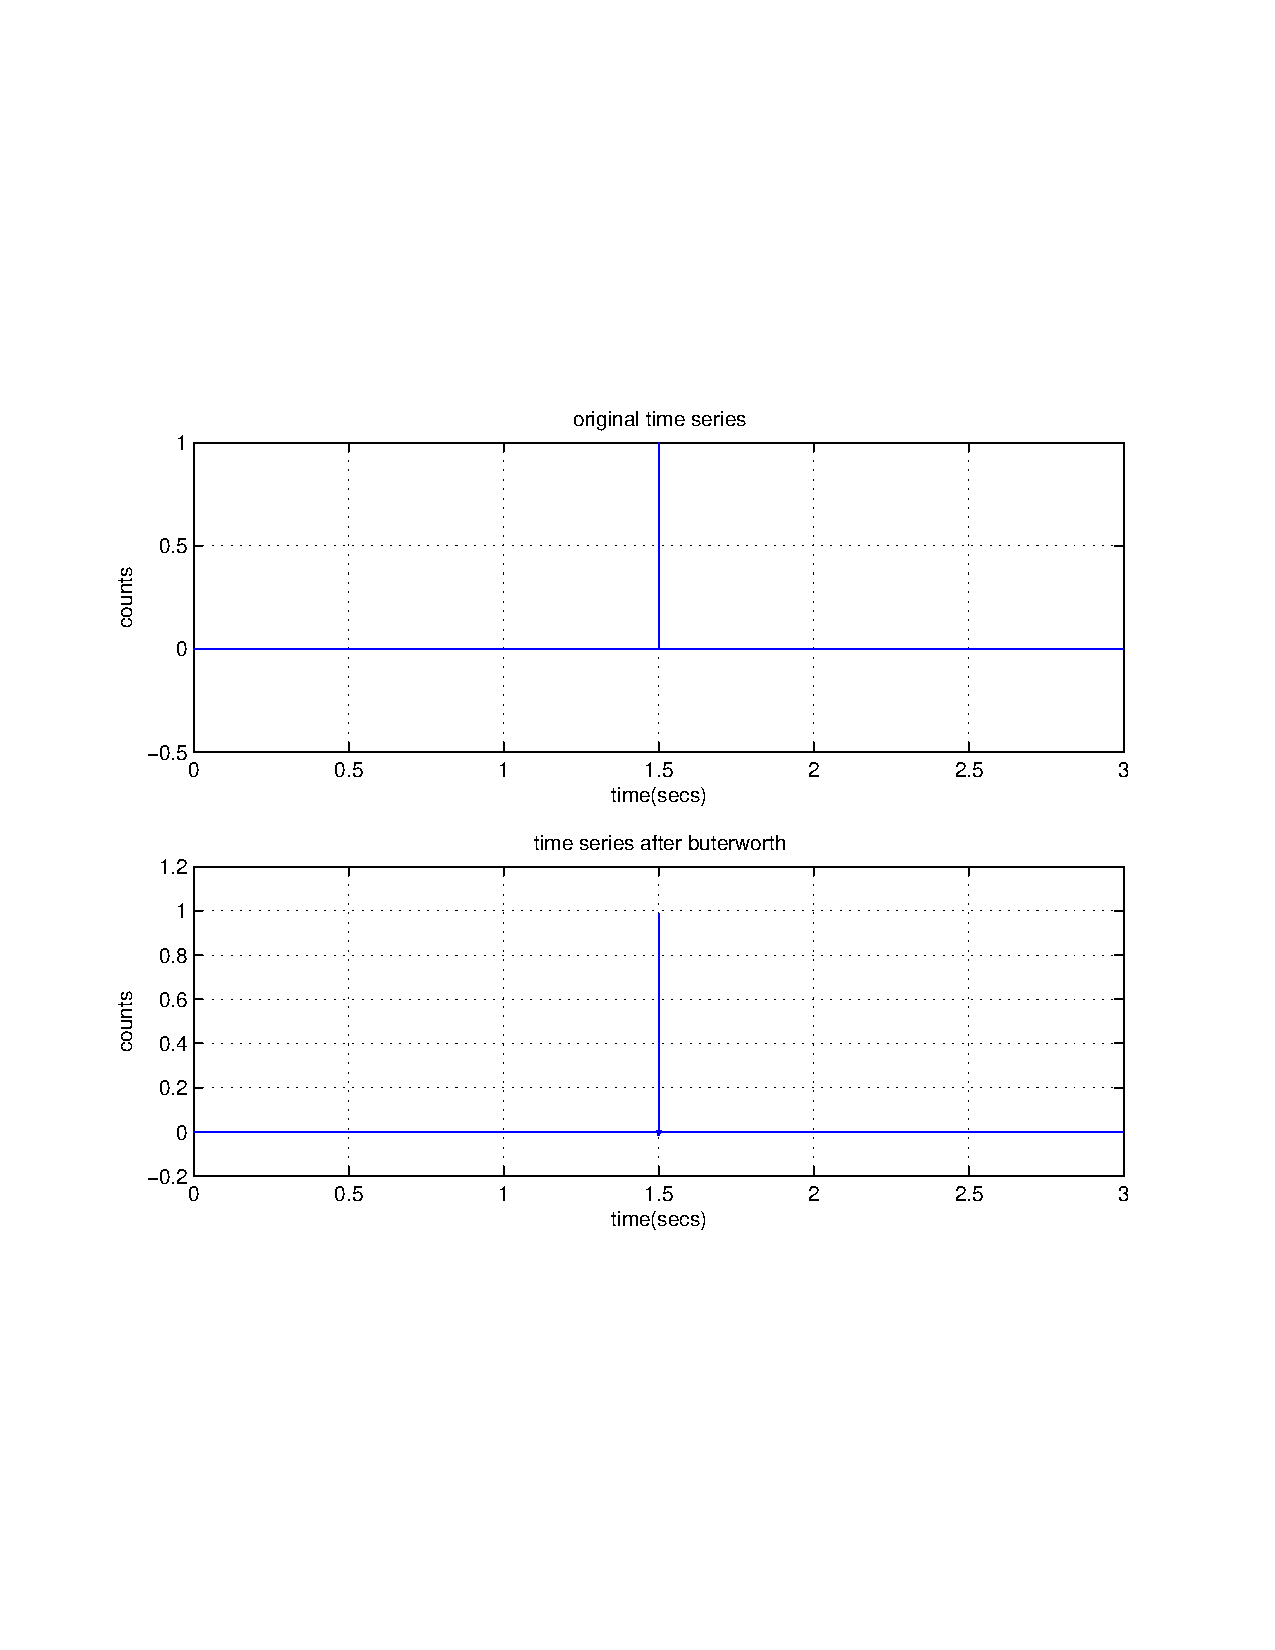
\includegraphics[width=0.9\textwidth]{figures/checkbuttertimeseries}
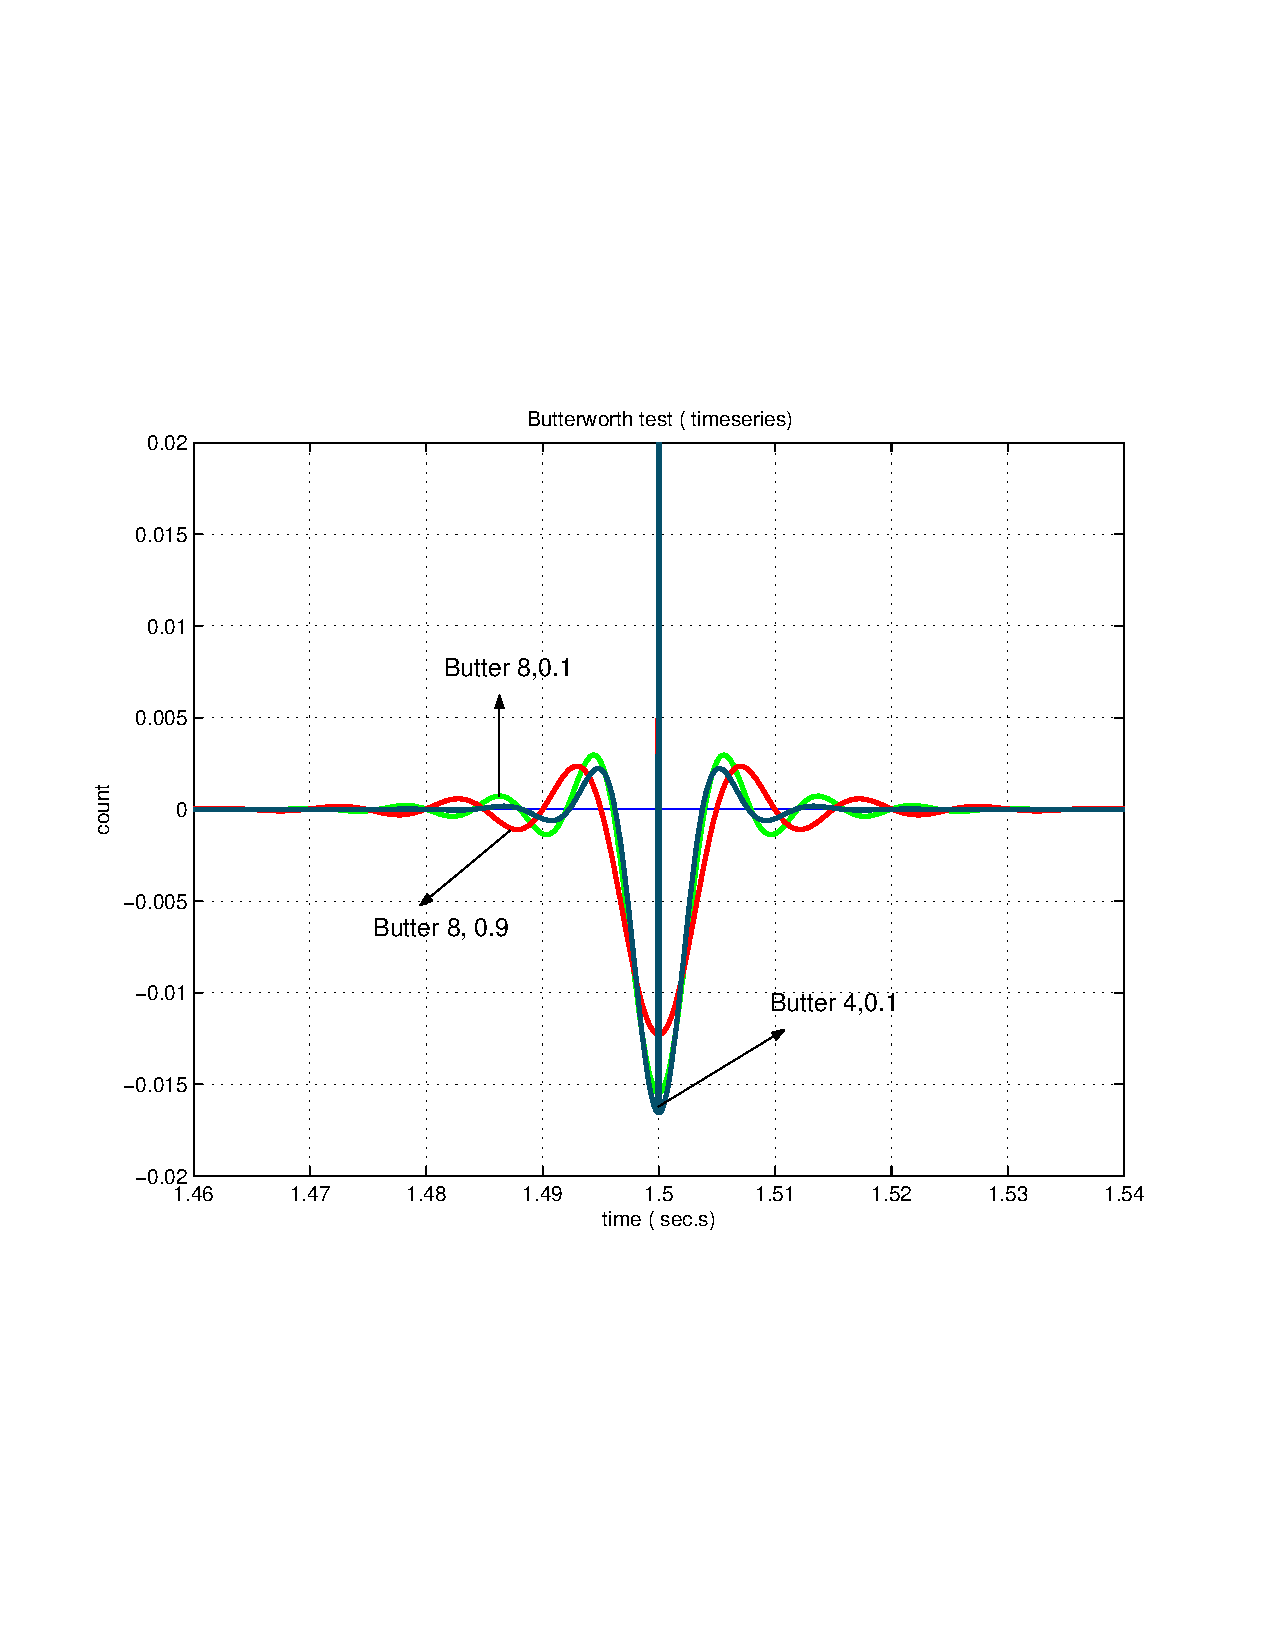
\includegraphics[width=0.9\textwidth]{figures/butter894comptimeseries}
\caption{Top panel: Time series before Butterworth and 
Bottom 2 panels: Time series after Butterworth} \label{fig:checkbuttertimeseries}
\end{center}
\end{figure}
The impulse response in Figure~\ref{fig:checkbuttertimeseries} shows  
time domain ringing produced by the filter. Maximum amplitude of 
the ringing is upto about $1.5$\% of the original time series amplitude.
However ringing in the side lobes die down to almost zero within about
20 milliseconds on both sides of the $\delta$ function. This ringing may
affect the timing resolution in real search, but we are yet
to quantify that effect.  

The Butterworth filter is created using the LAL routine,
\texttt{LALButterworthREAL4TimeSeries()} which uses the following 
parameters to specify the filter:
\begin{itemize}
  \item the low frequency cut off, f2. 
  \item The attenuation at f2. It gives a measure of power
    that is allowed to pass at f2.
  \item The filter order, nMax.
\end{itemize}

The frequency response of the filter is shown in Figure~\ref{fig:butterworthtest4} 
where the chosen parameters were $f2 = 120Hz$, $a2 = 0.1$ and $nMax = 4$.
\begin{figure}[h]
\centering
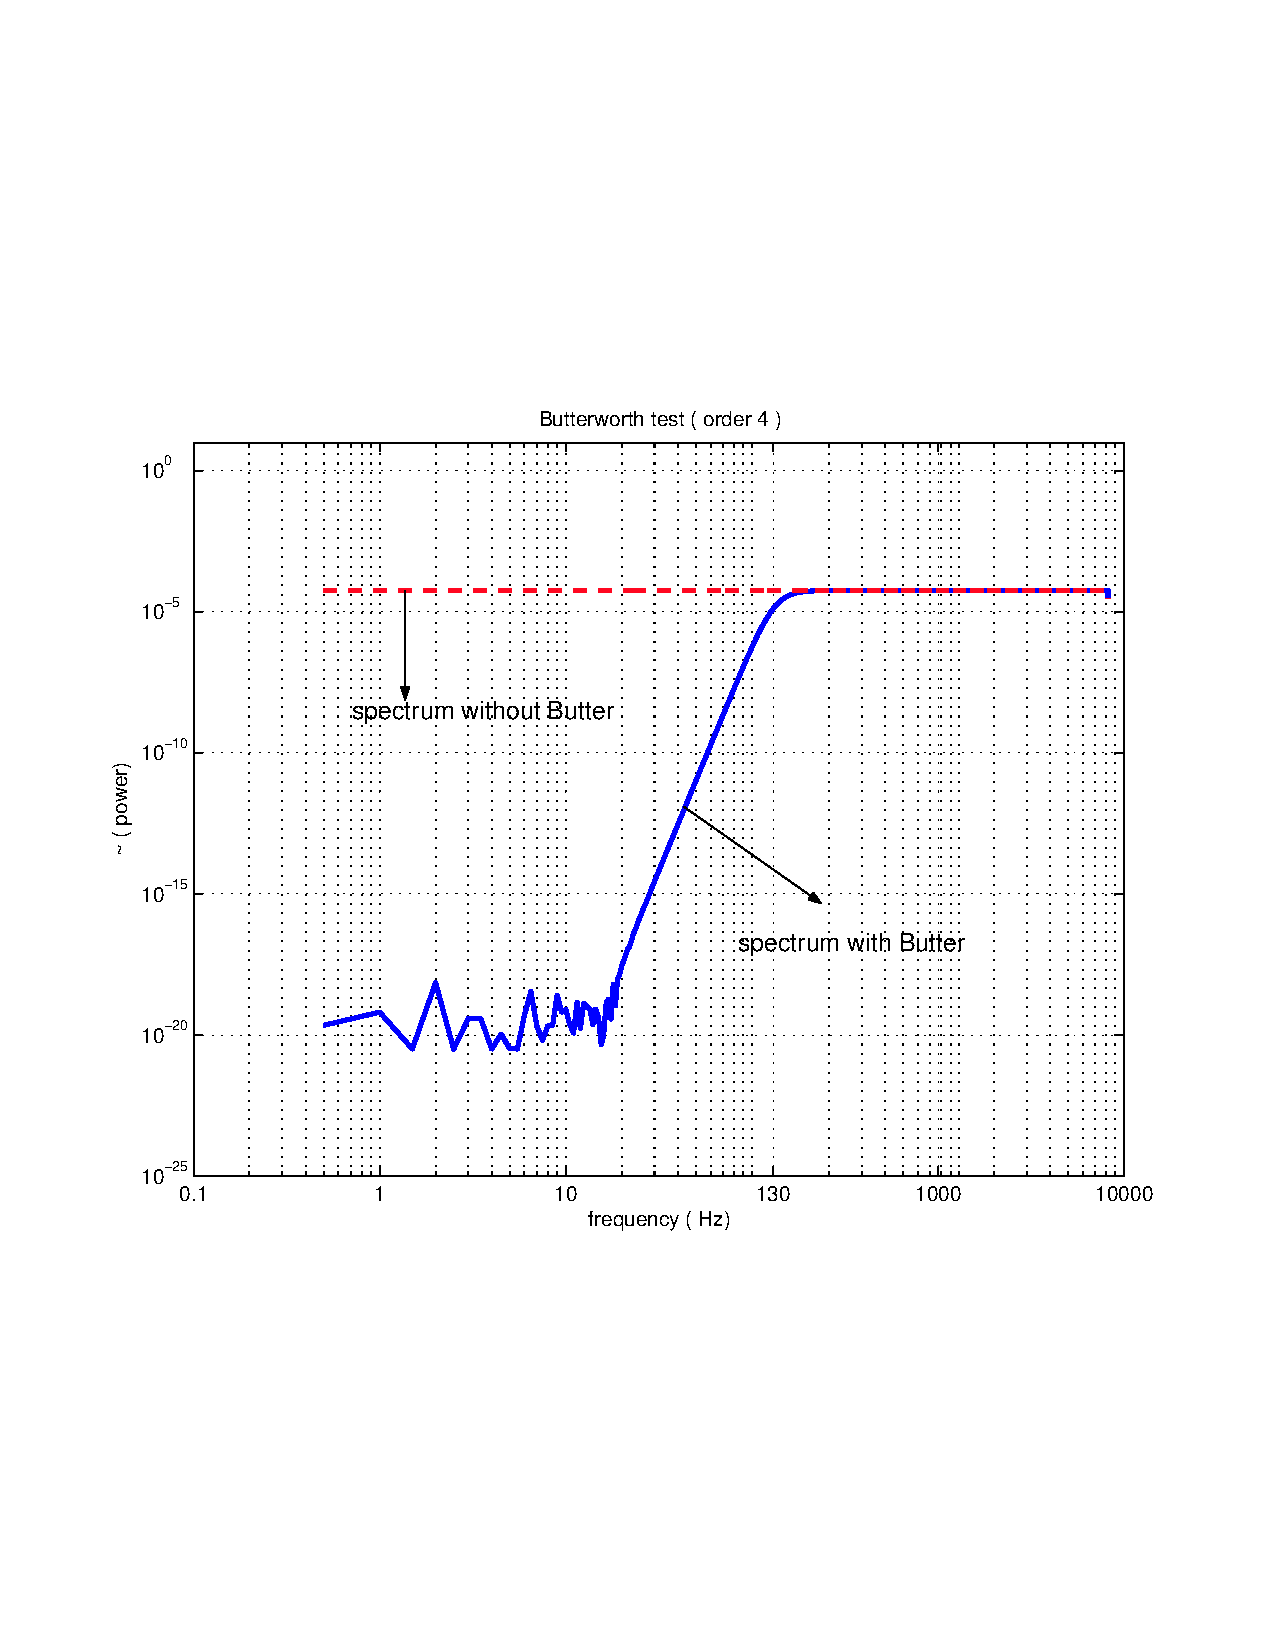
\includegraphics[width=0.9\textwidth]{figures/butterworthtest4}
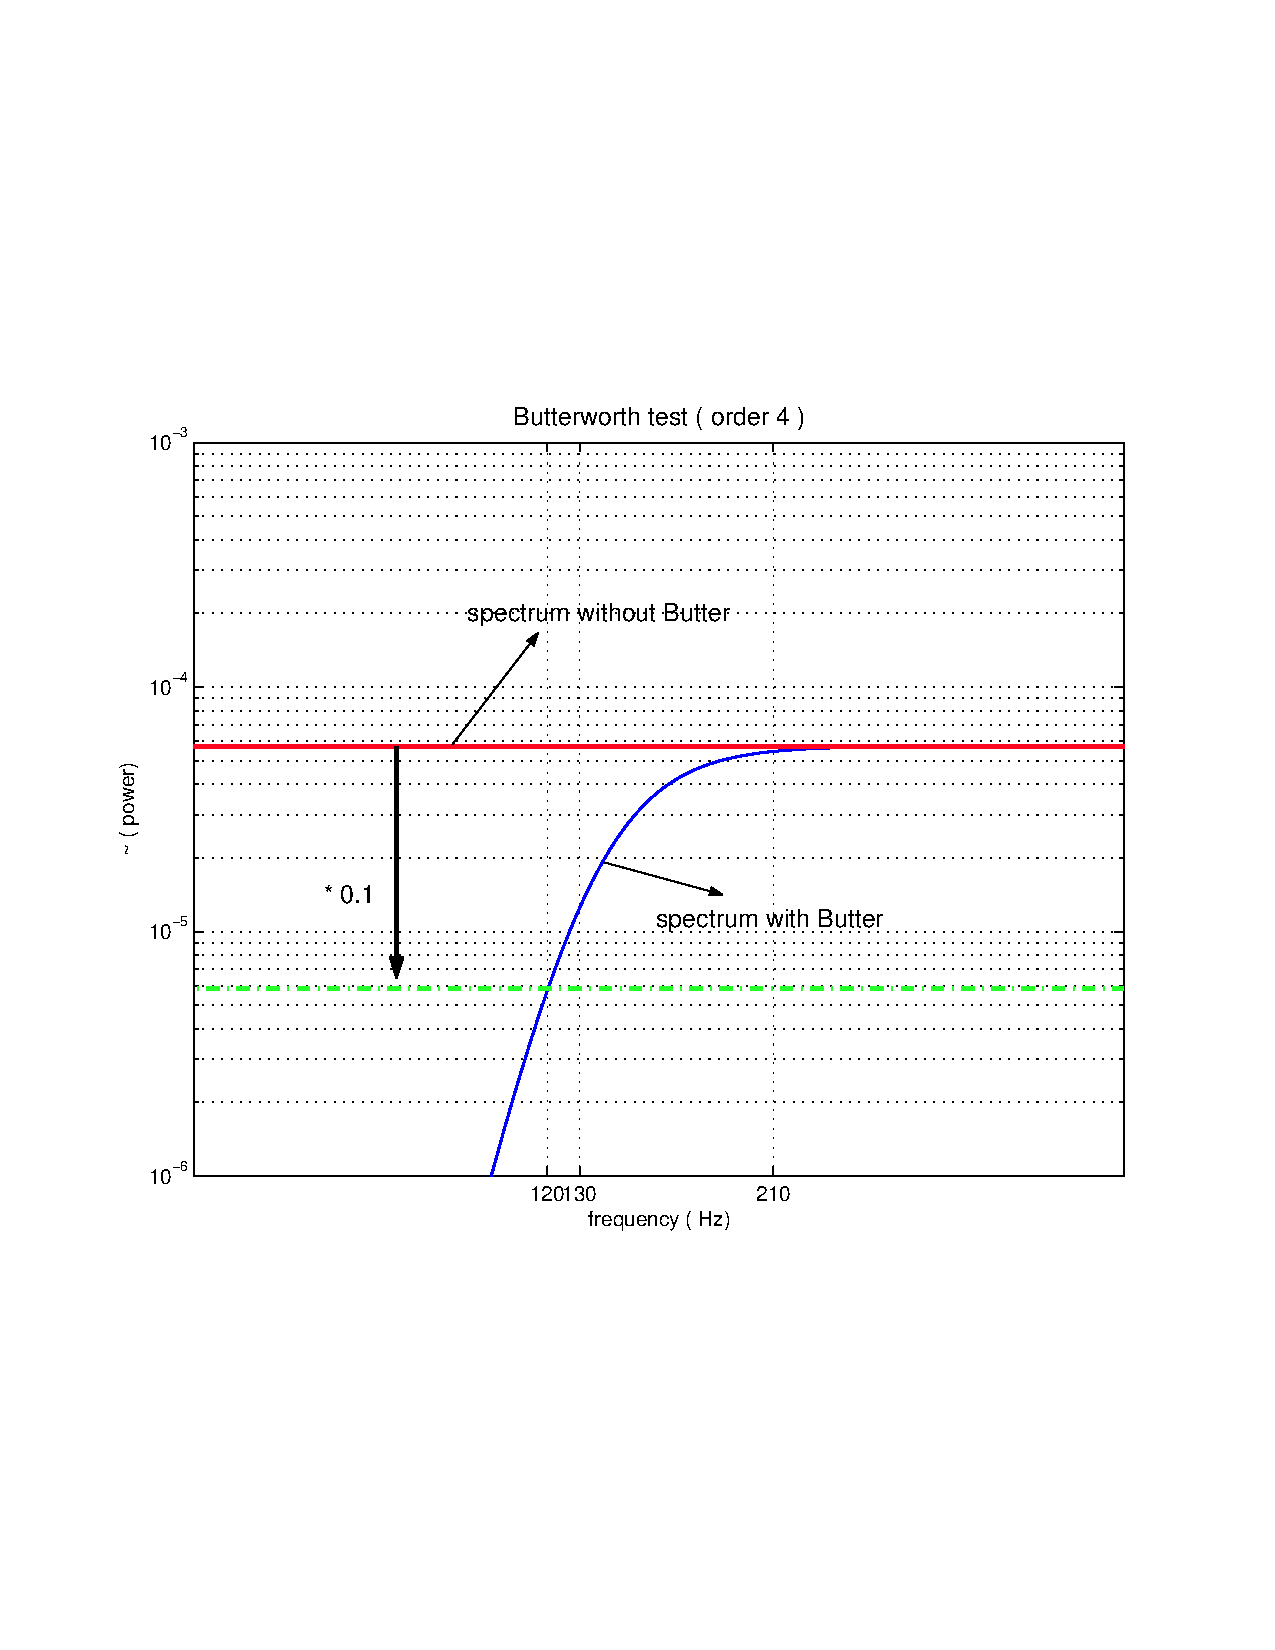
\includegraphics[width=0.9\textwidth]{figures/testattenuation4}
\caption{Frequency response of the high pass filter} \label{fig:butterworthtest4} 
\end{figure}
The red dotted line shows the spectrum which was measured without
the high pass filter while the blue line shows the spectrum after the data was 
high passed. From Figure~\ref{fig:butterworthtest4} 
it is evident that most of the frequency content below 100 Hz is being
blocked as desired. However this choice of parameters leeds to the 
undesirable feature that the signal power is suppressed all the way upto
$210$ Hz.                                         . 

The Excess Power code is configured to search for bursts above some 
minimal frequency, flow. It is therefore desirable to have little
or no attenuation above that frequency. The choice of Butterworth filter 
parameters that appear to achieve that are: 
\begin{itemize}
\item cutoff frequency,$f2 = flow - 10 Hz$
\item attenuatoin, $a2 = 0.9$
\item order, $Nmax = 8$
\end{itemize}
The frequency response of such a filter with $f2 = 120 Hz$ is shown in
Figure~\ref{fig:testattenuation8_9} 
\begin{figure}
\centering
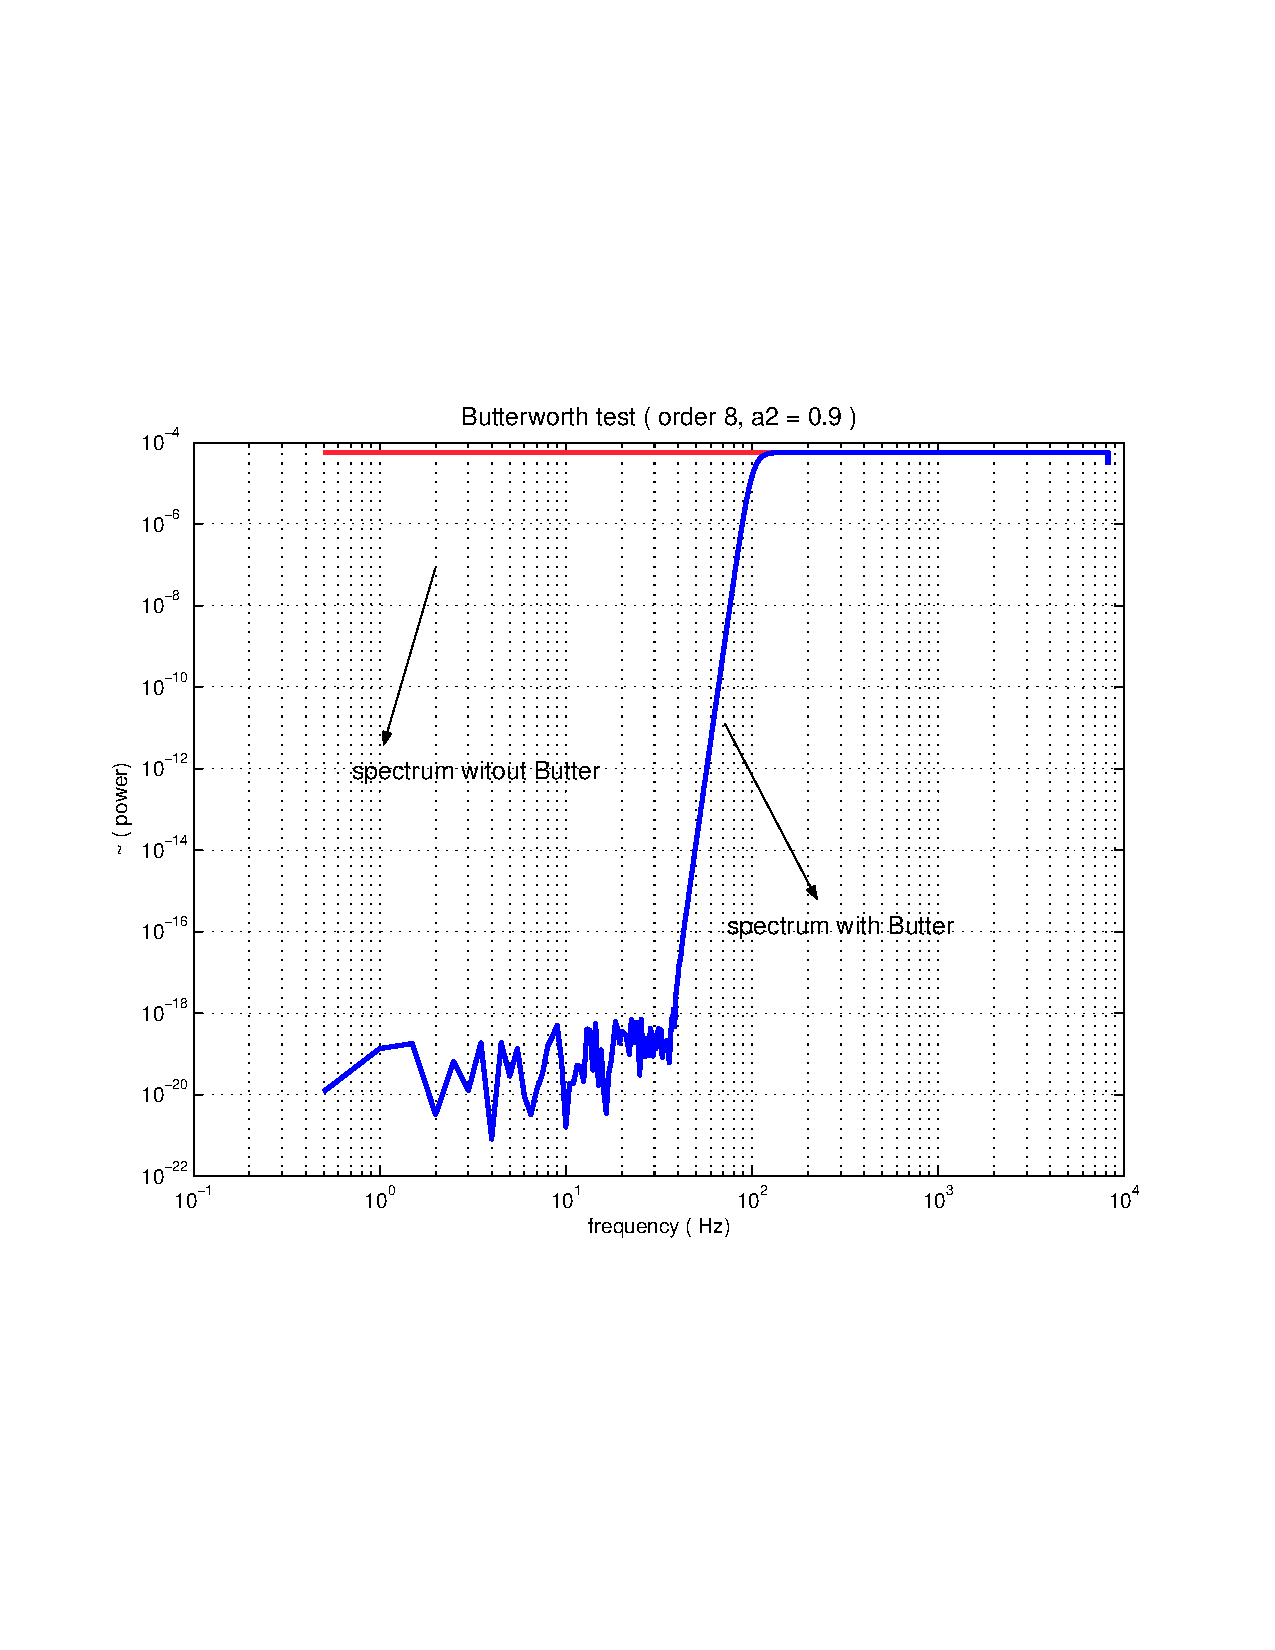
\includegraphics[width=0.9\textwidth]{figures/testattenuation8_9}
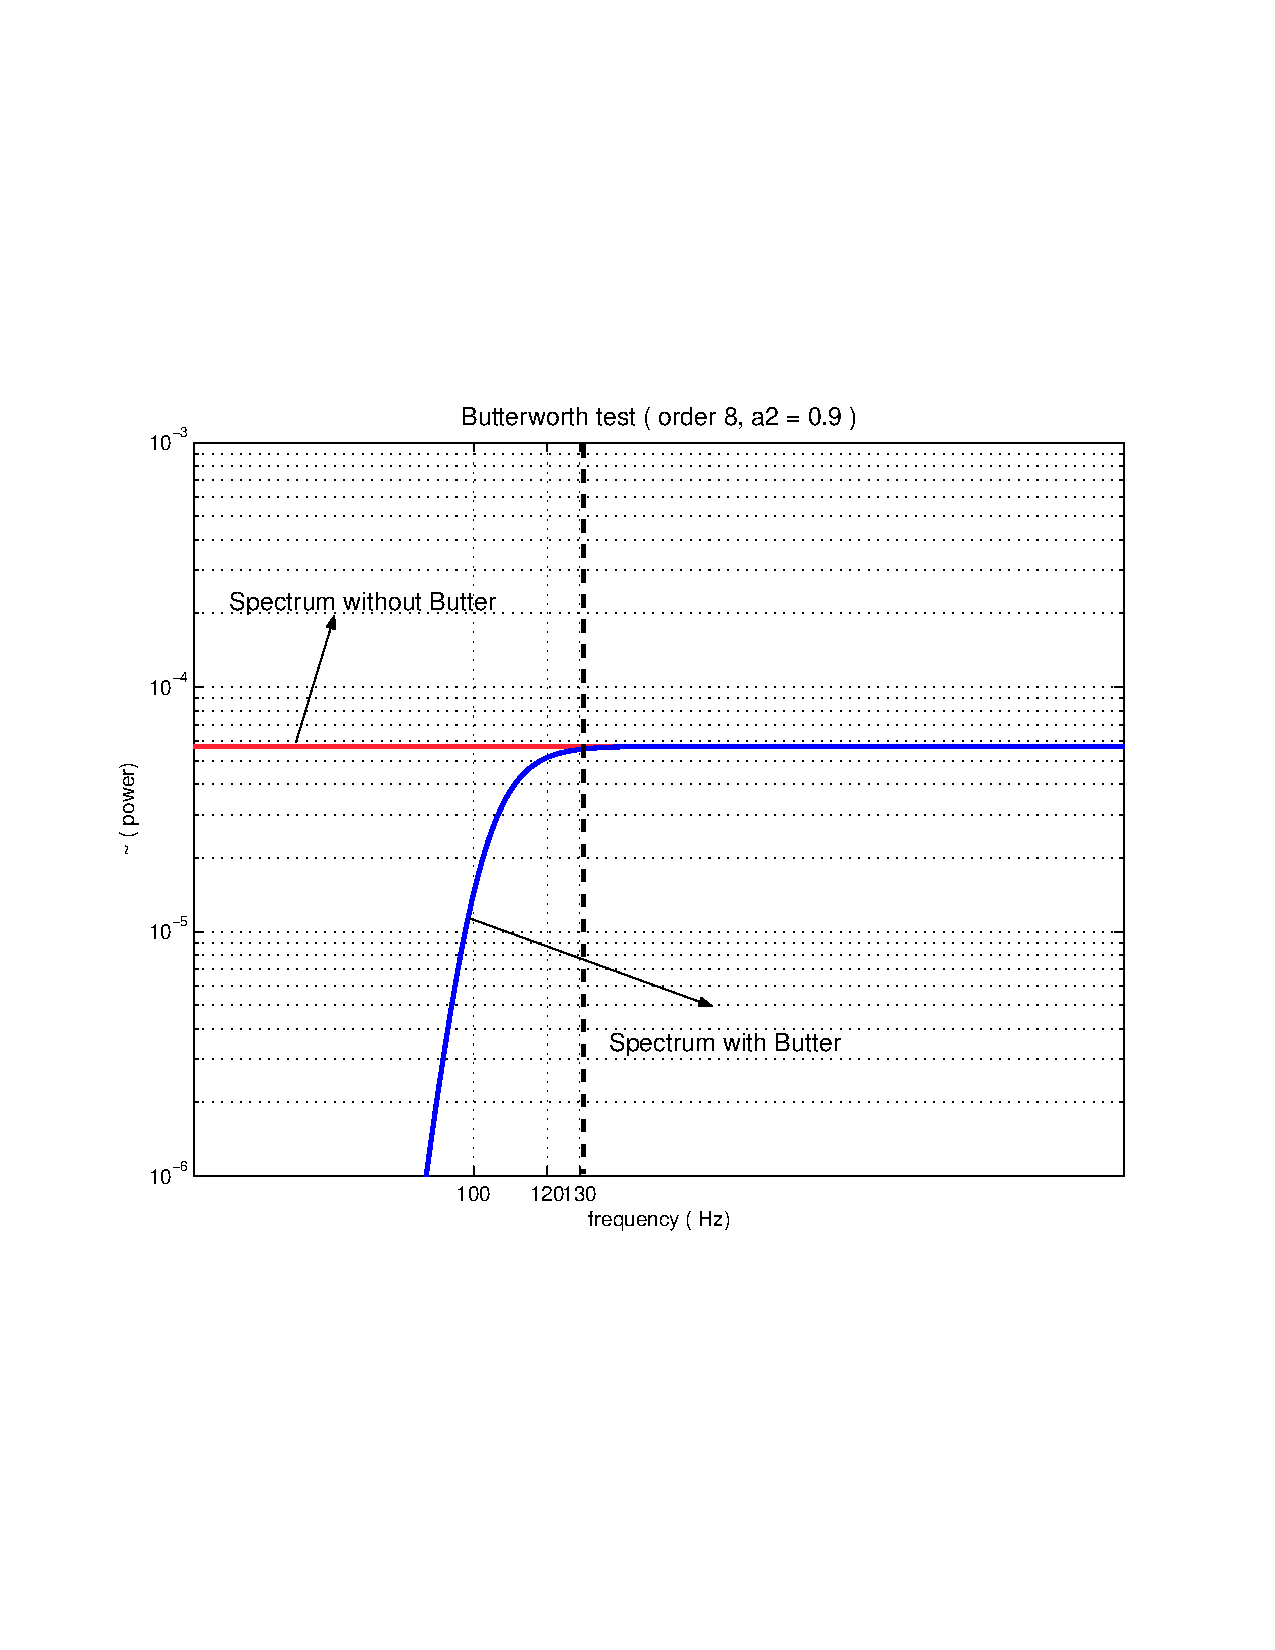
\includegraphics[width=0.9\textwidth]{figures/testattenuation8_9zoomed}
\caption{Comparison of the spectra: Filter order 8 and attenuation 0.9}
\label{fig:testattenuation8_9}
\end{figure}

\clearpage

%%%%%%%%%%%%%%%%%%%%%%%%%%%%%%%%%%%%%%%%%%%%%%%%%%%%%%%%%%%%%%%%%%%%%
% RUNNING A PIPELINE
%%%%%%%%%%%%%%%%%%%%%%%%%%%%%%%%%%%%%%%%%%%%%%%%%%%%%%%%%%%%%%%%%%%%%
\subsection{Running the power code under Condor}
\label{subsection:running_power}
\idx[Running]{power}

This section is under construction!


%%%%%%%%%%%%%%%%%%%%%%%%%%%%%%%%%%%%%%%%%%%%%%%%%%%%%%%%%%%%%%%%%%%%%%%%%%%%%%%
% subsection: power pipeline script
%%%%%%%%%%%%%%%%%%%%%%%%%%%%%%%%%%%%%%%%%%%%%%%%%%%%%%%%%%%%%%%%%%%%%%%%%%%%%%%
\clearpage
\subsection{Program \texttt{lalapps\_power\_pipe}}
\label{program:lalapps-power-pipe}
\idx[Program]{lalapps\_power\_pipe}

\begin{entry}

\item[Name]
\verb$lalapps_power_pipe$ --- builds a one interferometer
excess-power search DAG   

\item[Synopsis]
\verb$lalapps_power_pipe$ 
\verb$--mdccache$ \textsc{mdccache}
$\backslash$ \newline \hspace*{0.25in}
[\verb$--frame-cahce$ \textsc{frcache}]
\begin{verbatim}
  -h, --help               display this message
  -v, --version            print version information and exit
  -u, --user-tag TAG       tag the job with TAG (overrides value in ini file)

  -d, --datafind           run LSCdataFind to create frame cache files
  -r, --power              run lalapps_power on the first IFO

  -j, --injections FILE    add simulated bursts from FILE

  -p, --playground-only    only create chunks that overlap with playground
  -P, --priority PRIO      run jobs with condor priority PRIO

  -f, --config-file FILE   use configuration file FILE
  -l, --log-path PATH      directory to write condor log file
\end{verbatim}

\item[Description] 
\verb$lalapps_power_pipe$ builds an excess power search DAG suitable
for running at the various LSC Data Grid sites.   The script requires
a configuration file.   An example file can be found in
\verb+$LALPREFIX/share/lalapps/power_pipe.ini+    Arguments to be
passed to the search code are supplied in this file and used the DAG
construction.    This is a standard python format configuration file.

\item[Options]\leavevmode
\begin{entry}
\item[\texttt{--user-tag}  \textsc{tag}]   The tag for the job.  This
will override the value set in the ini file

\item[\texttt{--datafind}] run LSCdataFind as part of the DAG to
create the cache files for each science segment

\item[\texttt{--power}] run lalapps\_power on the data

\item[\texttt{--priority} \textsc{prio}] run jobs with condor priority PRIO

\item[\texttt{--config-file} \textsc{file}] use configuration file FILE

\item[\texttt{--log-path} \textsc{path}] directory to write condor log file
\end{entry}


\item[Example]
To run the program,  type:
\begin{verbatim}
 lalapps_power_pipe 
\end{verbatim}

\item[Author]
Duncan Brown, Patrick Brady and Saikat Ray-Majumder
\end{entry}
\clearpage


%%%%%%%%%%%%%%%%%%%%%%%%%%%%%%%%%%%%%%%%%%%%%%%%%%%%%%%%%%%%%%%%%%%%%%%%%%%%%%%
% subsection: power code
%%%%%%%%%%%%%%%%%%%%%%%%%%%%%%%%%%%%%%%%%%%%%%%%%%%%%%%%%%%%%%%%%%%%%%%%%%%%%%%
\clearpage
\subsection{Program \texttt{lalapps\_power}}
\label{program:lalapps-power}
\idx[Program]{lalapps\_power}

\begin{entry}

\item[Name]
\texttt{lalapps\_power} --- performs excess power analysis on real or
simulated data.

\newcommand{\function}[1]{\texttt{#1}}
\newcommand{\prog}[1]{\texttt{#1}}
\newcommand{\option}[1]{\texttt{#1}}
\newcommand{\parm}[1]{$<$\textit{#1}$>$}

\item[Synopsis]
\prog{lalapps\_power} \newline \hspace*{0.5in}
\option{--bandwidth}~\parm{bandwidth} \newline \hspace*{0.5in}
[\option{--calibration-cache}~\parm{cache file}] \newline \hspace*{0.5in}
\option{--channel-name}~\parm{string} \newline \hspace*{0.5in}
[\option{--cluster}] \newline \hspace*{0.5in}
[\option{--debug-level}~\parm{level}] \newline \hspace*{0.5in}
\option{--default-alpha}~\parm{alpha} \newline \hspace*{0.5in}
[\option{--event-limit}~\parm{count}] \newline \hspace*{0.5in}
\option{--filter-corruption}~\parm{samples} \newline \hspace*{0.5in}
\option{--frame-cache}~\parm{cache file} \newline \hspace*{0.5in}
\option{--frame-dir}~\parm{directory} \newline \hspace*{0.5in}
\option{--frame-sample-rate}~\parm{Hz} \newline \hspace*{0.5in}
[\option{--geodata}~\parm{high pass corner frequency}] \newline \hspace*{0.5in}
\option{--gps-end-time}~\parm{seconds} \newline \hspace*{0.5in}
\option{--gps-end-time-ns}~\parm{nanoseconds} \newline \hspace*{0.5in}
\option{--gps-start-time}~\parm{seconds} \newline \hspace*{0.5in}
\option{--gps-start-time-ns}~\parm{nanoseconds} \newline \hspace*{0.5in}
[\option{--help}] \newline \hspace*{0.5in}
[\option{--injection-file}~\parm{file name}] \newline \hspace*{0.5in}
\option{--low-freq-cutoff}~\parm{Hz} \newline \hspace*{0.5in}
[\option{--mdc-cache}~\parm{cache file}] \newline \hspace*{0.5in}
[\option{--mdc-channel}~\parm{channel name}] \newline \hspace*{0.5in}
\option{--min-freq-bin}~\parm{nfbin} \newline \hspace*{0.5in}
\option{--min-time-bin}~\parm{ntbin} \newline \hspace*{0.5in}
[\option{--noise-amplitude}~\parm{amplitude}] \newline \hspace*{0.5in}
\option{--nsigma}~\parm{sigma} \newline \hspace*{0.5in}
[\option{--printData}] \newline \hspace*{0.5in}
[\option{--printSpectrum}] \newline \hspace*{0.5in}
\option{--psd-average-method}~\parm{method} \newline \hspace*{0.5in}
\option{--psd-average-points}~\parm{samples} \newline \hspace*{0.5in}
[\option{--ram-limit}~\parm{MebiBytes}] \newline \hspace*{0.5in}
\option{--resample-filter}~\parm{filter type} \newline \hspace*{0.5in}
[\option{--seed}~\parm{seed}] \newline \hspace*{0.5in}
\option{--target-sample-rate}~\parm{Hz} \newline \hspace*{0.5in}
\option{--tile-overlap-factor}~\parm{factor} \newline \hspace*{0.5in}
\option{--threshold}~\parm{threshold} \newline \hspace*{0.5in}
[\option{--user-tag}~\parm{comment}] \newline \hspace*{0.5in}
[\option{--verbose}] \newline \hspace*{0.5in}
\option{--window}~\parm{window} \newline \hspace*{0.5in}
\option{--window-length}~\parm{samples} \newline \hspace*{0.5in}
\option{--window-shift}~\parm{samples}

\item[Description] 
\prog{lalapps\_power} performs an excess power analysis on real or
simulated data.  Consider searching for signals with the following
properties:
\begin{itemize}
\item Maximum signal time duration $T=2^a$ seconds where $a$ is a positive
or negative integer;  the sampling rate of the data stream is taken
assummed $\mbox{\texttt{srate}} = 2^b$ Hz.

\item The frequency band of the signal is between $f_{\mathrm{low}}$ Hz and
${f_{\mathrm{high}}}$ Hz.  Current versions of the code expect
${f_{\mathrm{high}}}-{f_{\mathrm{low}}}=2^d$ Hz where $d$ is an integer. 

\item Minimum time duration,

\item Minimum frequency bandwidth.
\end{itemize}

The input data for a search consists of LIGO/VIRGO \texttt{.gwf} frame
files.  These files can be collected together in a single directory, or in
locations described via the LAL frame cache file mechanism.  The code can
be used for Monte-Carlo simulations to determine search efficiency by
providing a list of injections to be made;  this injections list must be in
LIGO lightweight format and can be generated using the \prog{lalapps\_binj}
program described in Sec.~\ref{program:lalapps-binj}. 

The output data is written as \verb|sngl_burst| triggers in LIGO
lightweight XML files.  The files are named according to a standardized
naming convention
\begin{quote}
\{IFO\}-\{comment\}-POWER-\{GPS Start Time\}-\{duration\}.xml
\end{quote}
For example, if a search was run on the Hanford 4km interferometer and
generated triiggers starting at 731488397 and the triggers cover 33 seconds
after that time,  then the file name would be 
\begin{quote}
H1-test\_this\_again-POWER-731488397-33.xml
\end{quote}
where the comment was ``test\_this\_again''.  Note that the comment should
not include spaces and should use underscores instead.

\item[Options]\leavevmode
\begin{entry}
\item[\option{--bandwidth} \parm{bandwidth}]
Set the bandwidth in which the search is to be performed.  The integer
parameter \parm{bandwidth} is related to the physical bandwidth by the
formula
\[
\mbox{\parm{bandwidth}}
   = T \times (f_{\mathrm{high} - f_{\mathrm{low}}}).
\]

\item[\option{--calibration-cache} \parm{cache file}]
Specify the location of calibration information.  \parm{cache file} gives
the path to a LAL-format frame cache file describing locations of
\texttt{.gwf} frame files that provide the calibration data ($\alpha$ and
$\beta$ coefficients) for the analysis.  Frame cache files are explained in
the ``framedata'' package in LAL.

\item[\option{--channel-name} \parm{string}]
Set the name of the data channel to analyze to \parm{string}.  This must
match the name of one of the data channels in the input frame files.  For
example, ``\verb|H2:LSC-AS_Q|''.

\item[\option{--cluster}]
Enable a clustering algorithm.  The result is the reduction of overlapping
triggers to a single trigger which covers a square time-frequency volume
which encompasses all overlapping trigger regions.   The signal-to-noise
and the confidence associated with a clustered trigger belong to the most
significant excess-power trigger in the cluster.  \emph{Note:}  The
algorithm is in a prototyping stage, and its behaviour is not robustly
tested.  Treat with care, and look at the code to insure you understand the
implication of enabling this option.

\item[\option{--debug-level} \parm{level}]
Sets the LAL debug level to \parm{level}.  The default value is
\texttt{LALMSGLVL2}.  A useful setting is 65 which turns off memory
padding, but keeps memory tracking and error messages.  If you want to turn
off memory tracking completely, then use 33.

\item[\option{--default-alpha} \parm{alpha}]
Set the default alpha value for tiles with sigma $<$ numSigmaMin to
\parm{alpha}.  See the LAL ``burstsearch'' package for details.

\item[\option{--event-limit} \parm{count}]
Limit the number of events reported in each time interval corresponding to
the PSD average length to \parm{count}.  The default value is 999.

\item[\option{--filter-corruption} \parm{samples}]
The input time series data is passed through a conditioning filter prior to
analysis.  Generally, the conditioning filter should be expected to corrupt
some amount of the beginning and end of the time series due to edge
effects.  This parameter tells the code how much data, in samples, should
be ignored from the start and end of the time series.  A reasonable value
is 0.5 seconds worth of data.

\item[\option{--frame-cache} \parm{cache file}]
Obtain the locations of input \texttt{.gwf} frame files from the LAL frame
cache file \parm{cache file}.  LAL frame cache files are explained in the
``framedata'' package in LAL and can be constructed by making calls to
\prog{LSCDataFind} on some systems.  If both \option{--frame-cache} and
\option{--frame-dir} are specified, \option{--frame-dir} will be used.  If
neither \option{--frame-cache} nor \option{--frame-dir} are provided, then
\option{--noise-amplitude} must be given in order to force the creation of
simulated noise.

\item[\option{--frame-dir} \parm{directory}]
Use the \texttt{.gwf} frame files found in \parm{directory} for input.  If
both \option{--frame-cache} and \option{--frame-dir} are specified,
\option{--frame-dir} will be used.  If neither \option{--frame-cache} nor
\option{--frame-dir} are provided, then \option{--noise-amplitude} must be
given in order to force the creation of simulated noise.

\item[\option{--frame-sample-rate} \parm{Hz}]
Set the sample rate of the data found in the input frame files to \parm{Hz}
samples per second.  \emph{Note:} This parameter must match the actual data
rate found in the files;  the code's behaviour is undefined if this
condition is not met.  The existance of this parameter is an unfortunate
side-effect of the code's input logic, and there is an on-going effort to
remove the need to specify this information on the command line.  A future
version of this program will be able to obtain this information directly
from the input files.

\item[\option{--geodata} \parm{high pass corner frequency}]
Enable the processing of data from the GEO detector.  Data from the GEO
detector is not high-pass filtered and is stored in IEEE double-precision
format.  This program uses IEEE single-precision internally, so the
low-frequency noise present in the original data needs to be removed prior
to the reduction of sample precision or signal fidelity will be lost.
\parm{high pass corner frequency} sets the cut-off frequency of the
high-pass filter to be used.

\item[\option{--gps-end-time} \parm{seconds}]
Set the integer part of the GPS time up to which input data should be read
to \parm{seconds}.

\item[\option{--gps-end-time-ns} \parm{nanoseconds}]
Set the fractional part of the GPS time up to which input data should be
read to \parm{nanoseconds}.

\item[\option{--gps-start-time} \parm{seconds}]
Set the integer part of the GPS time from which to start reading input data
to \parm{seconds}.

\item[\option{--gps-start-time-ns} \parm{nanoseconds}]
Set the fractional part of the GPS time from which to start reading input
data to \parm{seconds}.

\item[\option{--help}]
Display a usage message and exit.

\item[\option{--injection-file} \parm{file name}]
Use \parm{file name} as a LIGO lightweight XML file containing a list of
injections to be made.   The file should contain a \verb+sim_burst+ table
which is used to set information about the types of injections to be made.
This file may be constructed by hand, or one can use the
\verb+lalapps_binj+ program described in Section
\ref{program:lalapps-binj}.   

\item[\option{--low-freq-cutoff} \parm{Hz}]
Set the lowest frequency at which to search for gravitational waves to
\parm{Hz}.  This parameter is $f_{\mathrm{low}}$ from our description of
the desired signal parameters above.

\item[\option{--mdc-cache} \parm{cache file}]
Use \parm{cache file} as a LAL format frame cache file describing the
locations of MDC frames to be used for injections.

\item[\option{--mdc-channel} \parm{channel name}]
Use the data found in the channel \parm{channel name} in the MDC frames for
injections.

\item[\option{--min-freq-bin} \parm{nfbin}]
Set the smallest extent in frequency of TF tiles to search to the integer
\parm{nfbin}.  A reasonable value for this parameter is $2$.  The product
$\mbox{\textsc{minfbin}} \times \mbox{\textsc{mintbin}}$ is the minimum
time-frequency volume to be searched.  See LAL ``burstsearch'' package for
details.

\item[\option{--min-time-bin} \parm{ntbin}]
Set the smallest extent in time of TF tiles to search to the integer
\parm{ntbin}.  A reasonable value for this parameter is $2$.   The product
$\mbox{\textsc{minfbin}} \times \mbox{\textsc{mintbin}}$ is the minimum
time-frequency volume to be searched.  See LAL ``burstsearch'' package for
details.

\item[\option{--noise-amplitude} \parm{amplitude}]
If this parameter is provided, then Gaussian white noise will be mixed with
the input data.  If neither \option{--frame-cache} nor \option{--frame-dir}
is provided, then the noise will be the only data analyzed.

\item[\option{--nsigma} \parm{sigma}]
The threshold of the number of sigma to the floating point number
\parm{sigma}.  See the LAL ``burstsearch'' package for details.

\item[\option{--printData}]
Print the input time series at various stages of conditioning to data files
for diagnostic purposes.  Generally a version of the input time series is
dumped before and after each round of injections is made.

\item[\option{--printSpectrum}]
Print the average PSD measured over each PSD interval as well as the
frequency-domain representation of each analysis window to data files.
This is used for diagnostics.

\item[\option{--psd-average-method} \parm{method}]
Set the averaging method used in determining the average power spectral
density to \parm{method}.  This can be one of ``useMean'', ``useMedian'',
or ``useUnity''.

\item[\option{--psd-average-points} \parm{samples}]
Use \parm{samples} samples from the input time series to estimate the
average power spectral density of the detector's noise.  The average PSD is
used to whiten the data prior to applying the excess power statistic.  The
number of samples used for estimating the average PSD must be commensurate
with the analysis window length and analysis window spacing --- i.e.\ an
integer number of analysis windows must fit in the data used to estimate
the average PSD --- however this program will automatically round the
actual number of samples used down to the nearest integer for which this is
true.  This elliminates the need of the user to carefully determine a valid
number for this parameter, allowing him/her to instead select a number that
matches the observed length of time for which the instrument's noise is
stationary.

\item[\option{--ram-limit} \parm{MebiBytes}]
The start and stop GPS times may encompass a greater quantity of data than
can be analyzed at once due to RAM limitations.  This parameter can be used
to tell the code how much RAM, in MebiBytes, is available on the machine,
which it then uses to heursitically guess at a maximum time series length
that should be read.  The code then loops over the input data, processing
it in chunks of this size, until it has completed the analysis.  If this
parameter is not supplied, then the entire time series for the segment
identified by the GPS start and end times will be loaded into RAM.

\item[\option{--resample-filter} \parm{filter type}]
Set the type of filter used in the data rate down-conversion to
\parm{filter type}.  This can be ``butterworth'' or ``ldas''.

\item[\option{--seed} \parm{seed}]
When mixing noise into the input data, use \parm{seed} to seed the random
number generator.

\item[\option{--target-sample-rate} \parm{Hz}]
Down-convert the input data stream to a sample rate of \parm{Hz} samples
per second prior to analysis.  This can be used to reduce the number of CPU
cycles required to analyze a given quantity of input data.  \emph{Note:}
All other parameters are given with respect to \emph{this} sample rate.
For example, the number of samples used to estimate the average PSD as
given by \option{--psd-average-points} refers to the time series following
date rate down-conversion.

\item[\option{--tile-overlap-factor} \parm{factor}]
This parameter influences the amount of overlap between neighboring
time-frequency tiles.  It must be an integer.  A reasonable value for this
parameter is 3.  See the LAL ``burstsearch'' package for more information.

\item[\option{--threshold} \parm{threshold}]
Set the threshold in alpha for which above which identified events should
be discarded.  See the LAL ``burstsearch'' package for details.

\item[\option{--user-tag} \parm{comment}]
Set the user tag to the string \parm{comment}.  This string must not
contain spaces or dashes (``-'').  underscores.  This string will appear in
the name of the file to which output information is written, and is
recorded in the various XML tables within the file.

\item[\option{--verbose}]
Enable the output of informational messages.

\item[\option{--window} \parm{window}]
Set the type of window to use when extracting an analysis window from the
time series to the LAL window corresponding to the integer parameter
\parm{window}.  See the LAL package ``window'' for a description of the
window that corresponds to each value of \parm{window}.

\item[\option{--window-length} \parm{samples}]
Set the number of samples to use for an analysis window to \parm{samples}.
Only the central half of the window will be analyzed, the first quarter and
last quarter of the window are used as padding to avoid corruption at
certain stages of the analysis.  For example, if you wish the code to
analyze the data in 1 second windows, you need to set this parameter to the
number of samples corresponding to 2 seconds of data.

\item[\option{--window-shift} \parm{samples}]
Set the number of samples each analysis window is shifted with respect to
the previous window to \parm{samples}.  This is typically set to one
quarter of the window length (i.e.\ half the length of data that is
actually analyzed).

\end{entry}

\item[Time Domain Segmentation]
The excess power analysis code does not process the input data as a
continuous time series;  rather the time series is split into a sequence of
discrete ``analysis windows'', which are each analyzed individually.  To
account for the possibility of a burst event stradling the boundary between
two analysis windows, successive windows are staggered in such a way that
they overlap one another in time.  In this way, a burst event occuring on
the boundary of one window will (typically) be centred in the next.

Because edge effects at various stages of the analysis can corrupt the
beginning and end of the analysis window, the actual quantity of data
extracted from the input time series to form a window is twice the amount
that is analyzed.  Only results from the central half of the window are
retained, with the first and last quarters of each window being discarded.
The arrangement is shown in the following diagram.
\begin{center}
\begin{picture}(0,0)%
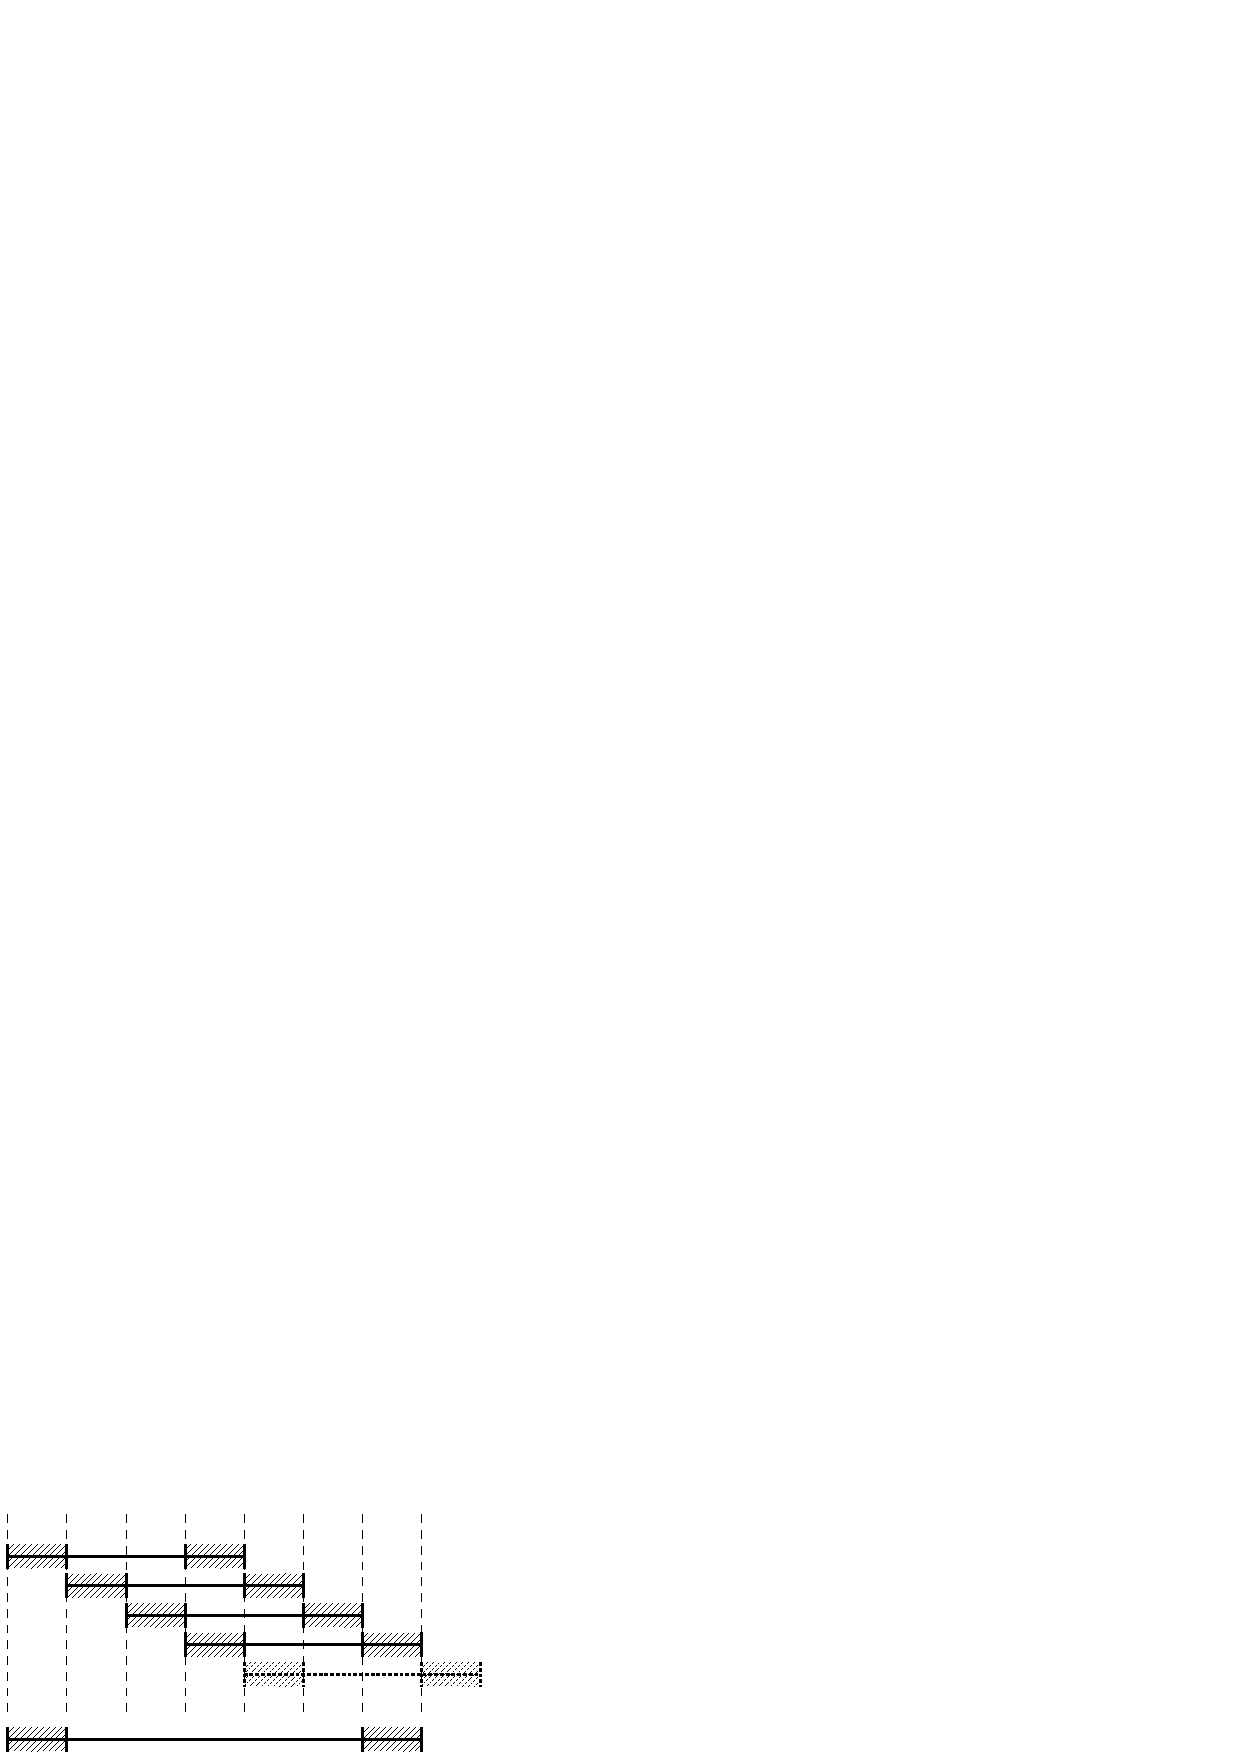
\includegraphics{figures/power/windows.fig.pdf}%
\end{picture}%
\setlength{\unitlength}{4144sp}%
%
\begingroup\makeatletter\ifx\SetFigFont\undefined%
\gdef\SetFigFont#1#2#3#4#5{%
  \reset@font\fontsize{#1}{#2pt}%
  \fontfamily{#3}\fontseries{#4}\fontshape{#5}%
  \selectfont}%
\fi\endgroup%
\begin{picture}(3194,1329)(-21,-253)
\put( 46,929){\makebox(0,0)[lb]{\smash{{\SetFigFont{10}{12.0}{\familydefault}{\mddefault}{\updefault}0}}}}
\put(1846,929){\makebox(0,0)[lb]{\smash{{\SetFigFont{10}{12.0}{\familydefault}{\mddefault}{\updefault}32768}}}}
\put(3151,434){\makebox(0,0)[lb]{\smash{{\SetFigFont{10}{12.0}{\familydefault}{\mddefault}{\updefault}\(\cdots\)}}}}
\end{picture}%

\end{center}
Here we see a discrete time series (represented by the bottom-most
horizontal line) that contains 57344 samples.  It has been divided into a
sequence of four analysis windows, each containing 32768 samples.  A fifth,
greyed-out, analysis window is shown to indicate where the next window in
the sequence would start.  In the analysis of each window, the first and
last 8192 samples (first and last quarter) are discarded as indicated by
the crossed-out sections in each window.  In this particular example, each
window is shifted 8192 samples (also equal to one quarter of the window
length) from the start of the previous window.  This choice of window
length and window shift causes the sections of each window that are
actually searched for events (the sections that are not crossed out) to
overlap their neighbours by half of their own width.  This is the typical
mode of operation for the search code.  Notice that the first and last
quarter window length of the complete time series (the cross-out sections
in the bottom line) are \emph{not} analyzed, as they are discarded from the
only analysis windows in which they appear.

The excess power code whitens the input time series using an estimate of
the instrument's noise power spectral density (PSD).  The estimated noise
PSD is computed by averaging the PSDs from a number of successive analysis
windows.  The noise PSD is not estimated by averaging over the entire time
series in order to allow the code to track the (possibly) changing
character of the instrument's noise.  For convenience, the user is
permitted to enter the number of samples that should be used to estimate
the PSD.  The number of samples entered should correspond to the time for
which the instrument's noise can be approximated as stationary for the
purpose of the excess power analysis.  Since, however, the actual
estimation procedure involves averaging over an integer number of analysis
windows, it is necessary for the number of samples selected to correspond
to the boundary of an analysis window.  For convenience,
\prog{lalapps\_power} will automatically round the value entered down to
the nearest analysis window boundary.

The LAL function \function{EPSearch()} performs the parts of the analysis
described above.  It is given a time series that it divides into analysis
windows, which it uses to estimate the noise PSD.  Using the estimated
noise PSD, it whitens each analysis window and then searches them for burst
events.  Only the analysis windows within the data used to estimate the
noise PSD are whitened using that estimate.  Once those windows have been
searched for burst events, \function{EPSearch()} returns to the calling
procedure which then extracts a new time series and the process repeats.
The parameter provided via the command line option
\option{--psd-average-points} sets the length of the time series that is
passed to \function{EPSearch()}.

As each successive time series is passed to \function{EPSearch()}, in order
for the analysis windows in the two time series to overlap each other
correctly --- i.e.\ to ensure the same overlap between analysis windows in
neighbouring time series as exists between neighbouring windows within a
series --- it is necessary for the second time series to begin
$(\mbox{\parm{window length}} - \mbox{\parm{window shift}})$ samples before
the end of the first series.  The arrangement is shown in the following
figure.
\begin{center}
\begin{picture}(0,0)%
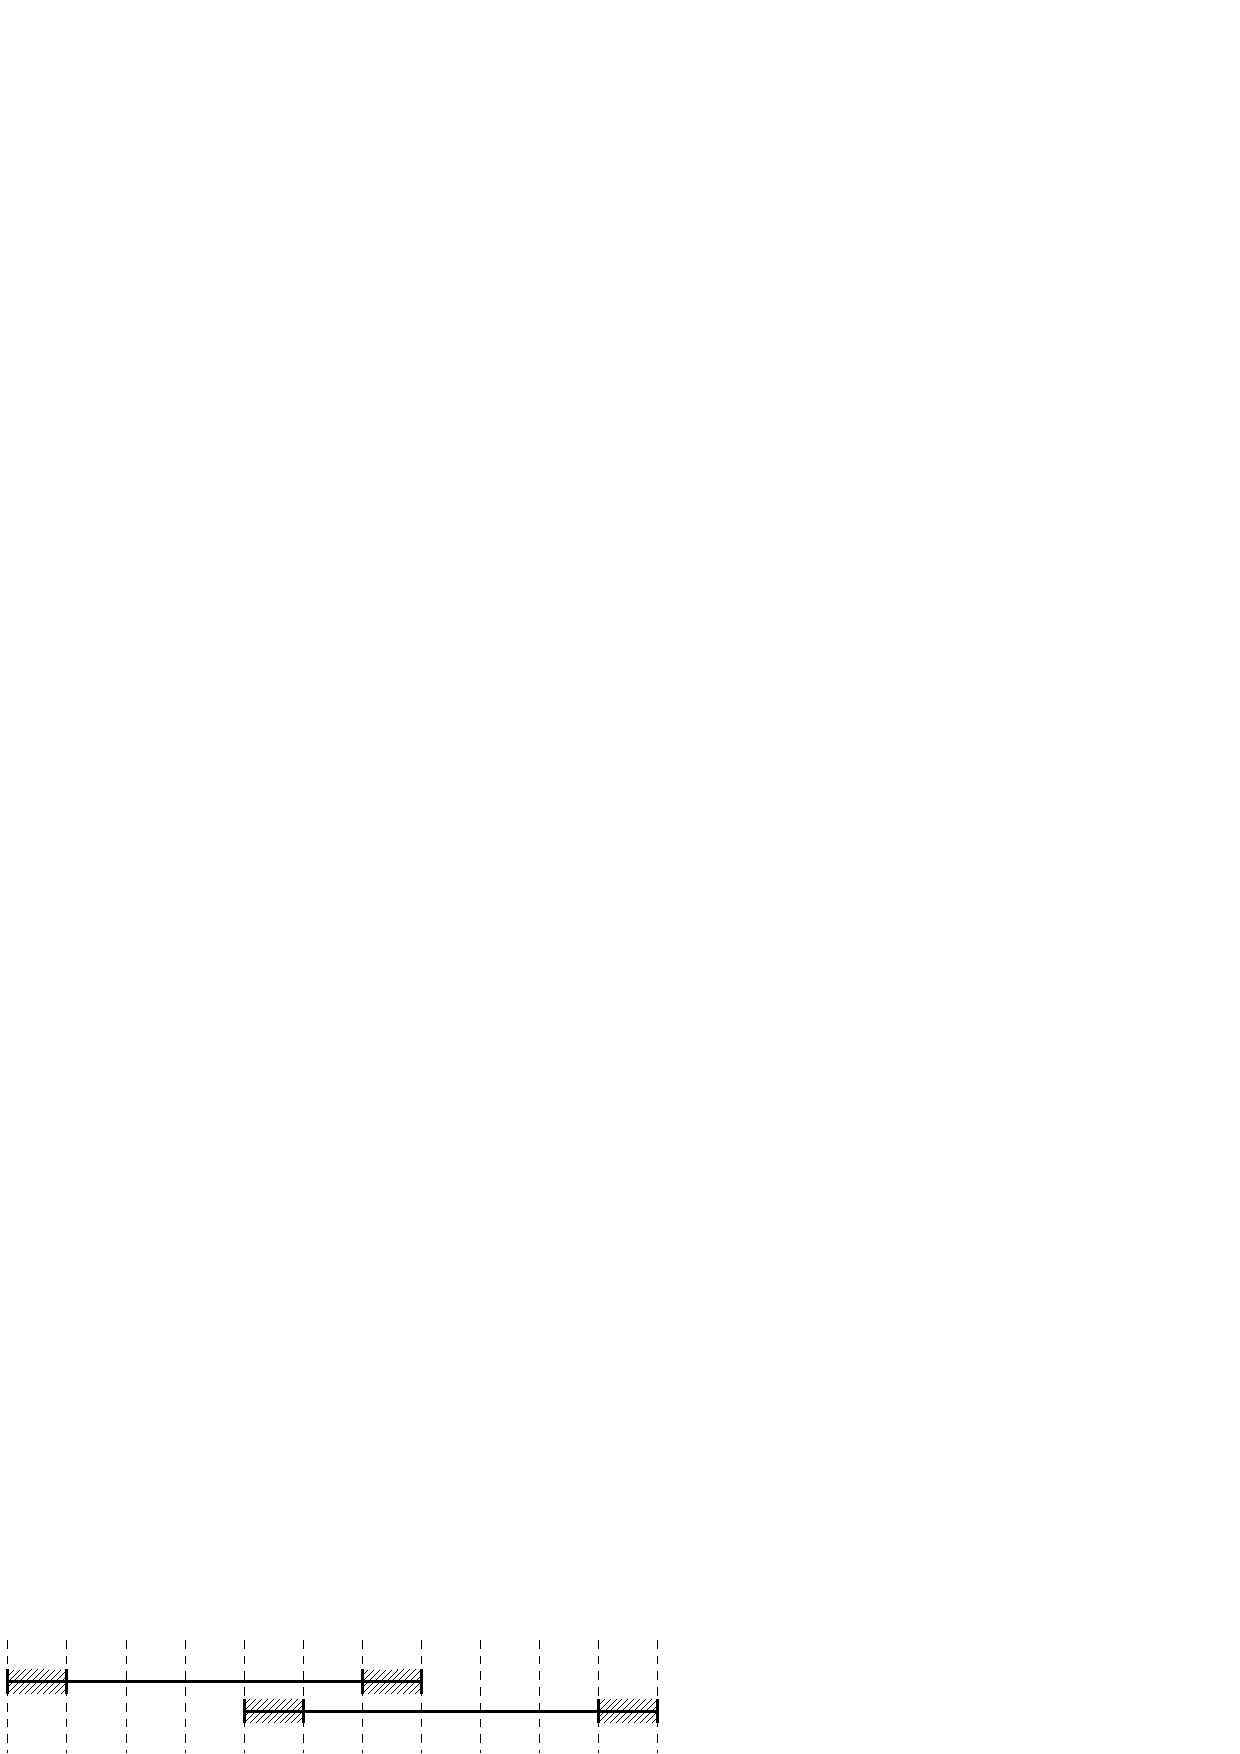
\includegraphics{figures/power/psds.fig.pdf}%
\end{picture}%
\setlength{\unitlength}{4144sp}%
%
\begingroup\makeatletter\ifx\SetFigFont\undefined%
\gdef\SetFigFont#1#2#3#4#5{%
  \reset@font\fontsize{#1}{#2pt}%
  \fontfamily{#3}\fontseries{#4}\fontshape{#5}%
  \selectfont}%
\fi\endgroup%
\begin{picture}(5364,1032)(-59,197)
\put(-44,1109){\makebox(0,0)[lb]{\smash{{\SetFigFont{10}{12.0}{\familydefault}{\mddefault}{\updefault}0}}}}
\put(1756,1109){\makebox(0,0)[lb]{\smash{{\SetFigFont{10}{12.0}{\familydefault}{\mddefault}{\updefault}32768}}}}
\put(3106,1109){\makebox(0,0)[lb]{\smash{{\SetFigFont{10}{12.0}{\familydefault}{\mddefault}{\updefault}57344}}}}
\put(4906,1109){\makebox(0,0)[lb]{\smash{{\SetFigFont{10}{12.0}{\familydefault}{\mddefault}{\updefault}90112}}}}
\end{picture}%

\end{center}
Here we see two of the time series from the first diagram above, each of
which is to be passed to \function{EPSearch()} for analysis.  To see why
the overlap between these two time series must be chosen as it is, refer to
the first diagram above to see where the greyed-out fifth analysis window
was to be placed.  That is where the first analysis window in the second
time series here will be placed.

Prior to looping over the data one noise PSD estimation length at a time,
the data is passed through a conditioning filter.  To account for edge
effects in the filter, an amount of data set by the command line option
\option{--filter-corruption} is dropped from the analysis at both the
begining and end of the time series.  The arrangement is shown in the
following diagram.
\begin{center}
\begin{picture}(0,0)%
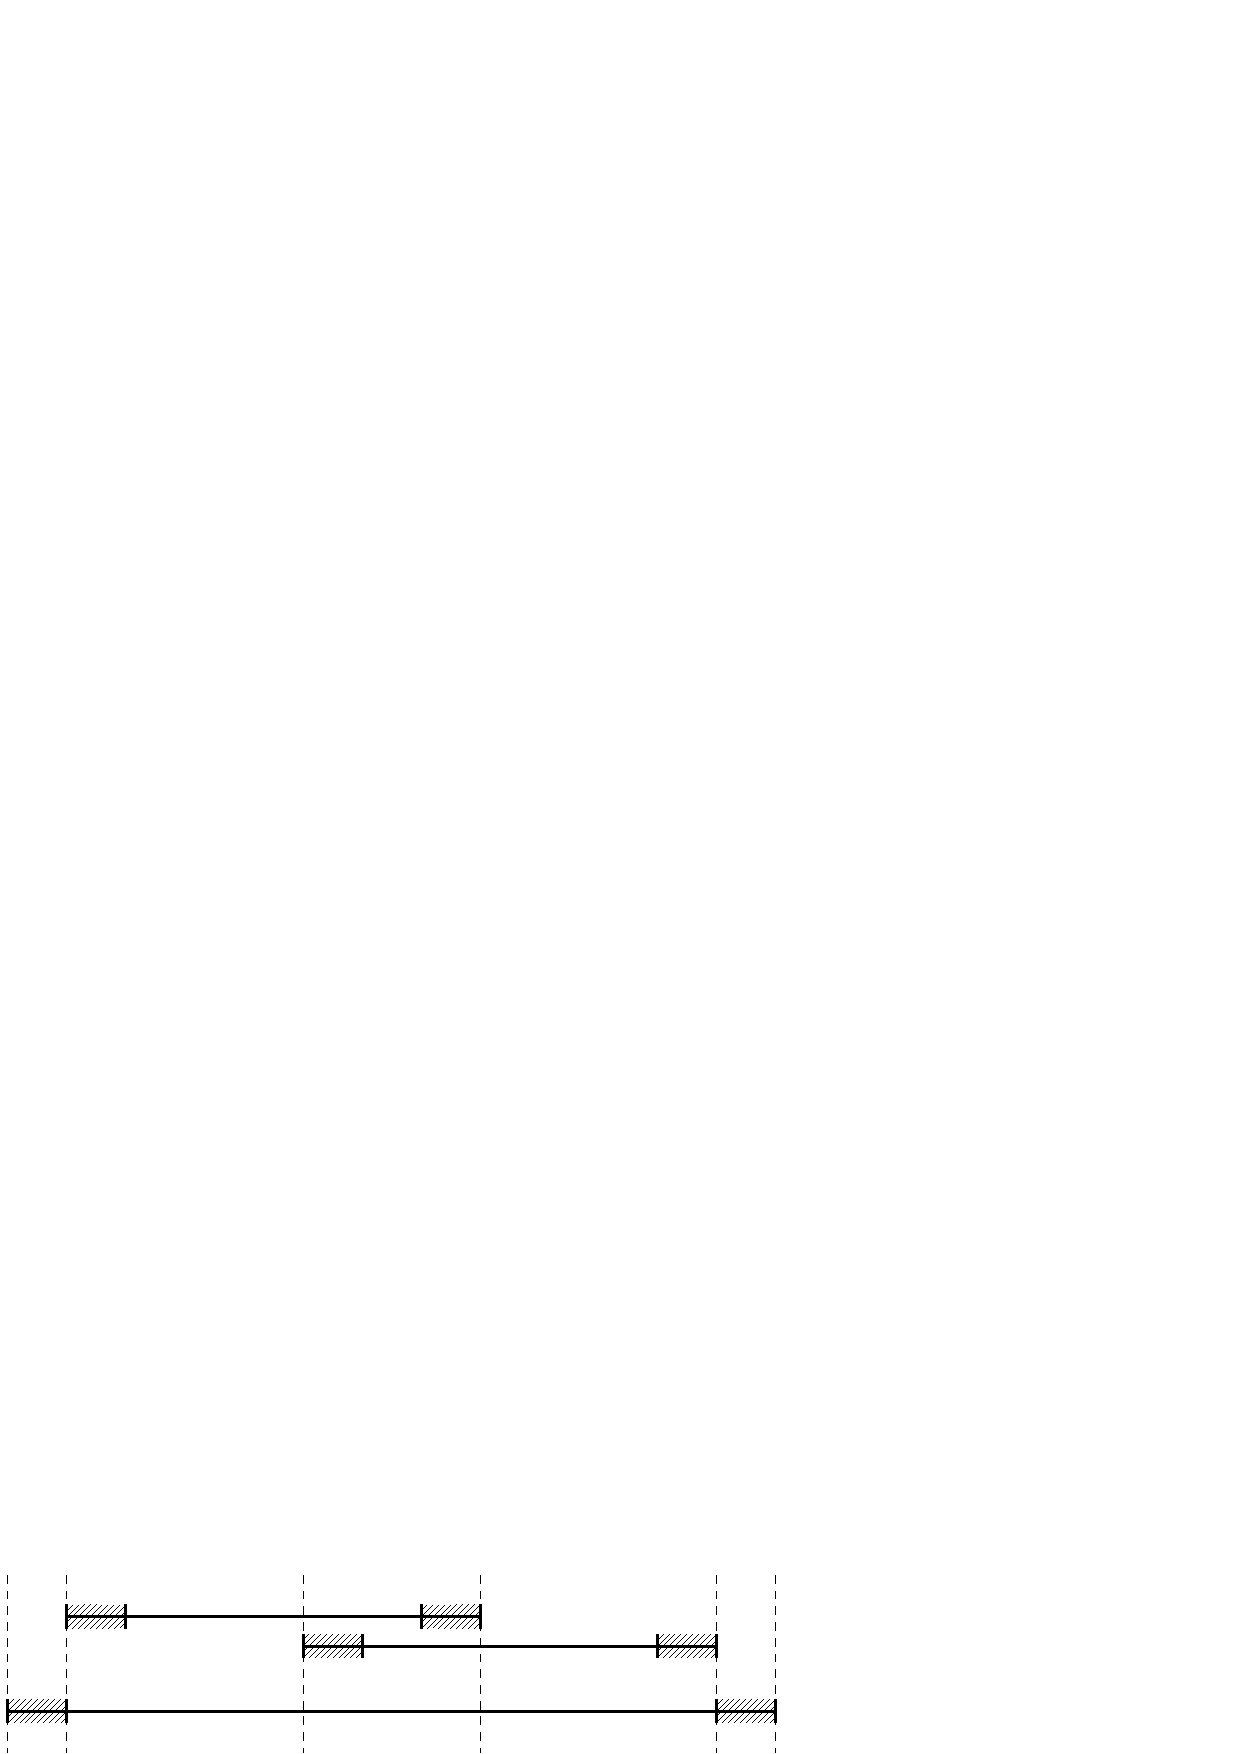
\includegraphics{figures/conditioning.fig.pdf}%
\end{picture}%
\setlength{\unitlength}{4144sp}%
%
\begingroup\makeatletter\ifx\SetFigFont\undefined%
\gdef\SetFigFont#1#2#3#4#5{%
  \reset@font\fontsize{#1}{#2pt}%
  \fontfamily{#3}\fontseries{#4}\fontshape{#5}%
  \selectfont}%
\fi\endgroup%
\begin{picture}(6341,1527)(-509,-298)
\put(-494,1109){\makebox(0,0)[lb]{\smash{{\SetFigFont{10}{12.0}{\familydefault}{\mddefault}{\updefault}0}}}}
\put(-44,1109){\makebox(0,0)[lb]{\smash{{\SetFigFont{10}{12.0}{\familydefault}{\mddefault}{\updefault}8192}}}}
\put(1756,1109){\makebox(0,0)[lb]{\smash{{\SetFigFont{10}{12.0}{\familydefault}{\mddefault}{\updefault}40960}}}}
\put(3106,1109){\makebox(0,0)[lb]{\smash{{\SetFigFont{10}{12.0}{\familydefault}{\mddefault}{\updefault}65536}}}}
\put(4906,1109){\makebox(0,0)[lb]{\smash{{\SetFigFont{10}{12.0}{\familydefault}{\mddefault}{\updefault}98304}}}}
\put(5356,1109){\makebox(0,0)[lb]{\smash{{\SetFigFont{10}{12.0}{\familydefault}{\mddefault}{\updefault}106496}}}}
\end{picture}%

\end{center}
The bottom-most line in this diagram represents the time series as read
into memory from disk.  In this example we have read 106496 samples into
memory, and after passing it through the conditioning filter 8192 samples
are dropped from the beginning and end of the series.  The remaining data
is then passed to \function{EPSearch()} 57344 samples at a time --- just as
was done in the earlier examples --- with appropriate overlaps.  In this
example, it happens that an integer number of overlaping noise PSD
intervals fits into the data that survives the conditioning.  In general
this will not be the case.  If the last noise PSD interval would extend
beyond the end of the time series, it is moved to an earlier time so that
its end is aligned with the end of the available data.

If more data needs to be analyzed than will fit in RAM at one time, we must
read it into memory and analyze it pieces.  In doing this, we again want
the analysis windows in neighbouring read cycles to overlap one another in
the same manner that neighbouring analysis windows within a single noise
PSD interval overlap one another.  This will be assured if, in the diagram
above, the start of the next data to be read from disk is arranged so that
the first noise PSD interval to be analyzed within it starts at the correct
location relative to the last PSD interval analyzed from the previous read
cycle.  Consideration of the diagram above reveals that in order to meet
this condition, the next data to be read into memory should start $(2
\mbox{\parm{filter corruption}} + \mbox{\parm{window length}} -
\mbox{\parm{window shift}})$ samples prior to the end of the previous data
to have been read.


\item[Example]
To run the program, type:
\begin{verbatim}
lalapps_power \
--bandwidth 1024 \
--channel-name "H1:LSC-AS_Q" \
--cluster \
--default-alpha 0.5 \
--filter-corruption 8192 \
--frame-cache H-754008315-754008371.cache \
--frame-sample-rate 16384 \
--gps-end-time 754008363 \
--gps-end-time-ns 0 \
--gps-start-time 754008323 \
--gps-start-time-ns 0 \
--low-freq-cutoff 130.0 \
--min-freq-bin 2 \
--min-time-bin 2 \
--nsigma 2.0 \
--psd-average-method useMedian \
--psd-average-points 548864 \
--resample-filter butterworth \
--target-sample-rate 16384 \
--threshold 1.0e-9 \
--tile-overlap-factor 3 \
--user-tag testing \
--verbose \
--window 2 \
--window-length 32768 \
--window-shift 8192
\end{verbatim}
For this to succeed, the current directory must contain the file
\texttt{H-754008315-754008931.cache} describing the locations of the
\texttt{.gwf} frame files with channel \verb|H1:LSC-AS_Q| data at 16384
samples per second for the GPS times 754008323.0 s through 754008363.0 s.

\item[Authors]
Patrick Brady,  Kipp Cannon and Saikat Ray Majumder 
\end{entry}
\clearpage

%%%%%%%%%%%%%%%%%%%%%%%%%%%%%%%%%%%%%%%%%%%%%%%%%%%%%%%%%%%%%%%%%%%%%
% BURCA:  coincidence analysis code
%%%%%%%%%%%%%%%%%%%%%%%%%%%%%%%%%%%%%%%%%%%%%%%%%%%%%%%%%%%%%%%%%%%%%
\subsection{Program \texttt{lalapps\_burca}}
\label{program:lalapps-burca}
\idx[Program]{lalapps\_burca}

\begin{entry}
\item[Name]
\verb$lalapps_burca$ --- program does burst coincidence analysis.

\item[Synopsis]
\verb$lalapps_burca$ 
\verb$--ifo-a$ \textsc{trigfile.a} \verb$--ifo-b$ \textsc{trigfile.b} 
[\verb$--start-time$ \textsc{startcoincidence}]
$\backslash$ \newline \hspace*{0.25in}
[\verb$--stop-time$ \textsc{endcoincidence}] 
[\verb$--drhoplus$ \textsc{drhoplus}] [\verb$--drhominus$ \textsc{drhominus}] 
$\backslash$ \newline \hspace*{0.25in}
[\verb$--dt$ \textsc{deltat}] 
\verb$--outfile$ \textsc{outfile} [\verb$--noplayground$] 
[\verb$--help$]

\item[Description] 
\verb$lalapps_burca$ performs coincidence on triggers from the burst
search code.  (At present it works for only two interferometers.) It
must be called with at least one input file from each instrument. The
default behavior outputs triggers during playground times to the file
\textsc{outfile};  to obtain all triggers,  use the
\verb$--noplayground$ flag.     
%Events can also be clustered
%within \textsc{msec} msec or a template bank for triggered searches
%can be constructed.

\item[Options]\leavevmode
\begin{entry}
\item[\texttt{--ifo-a} \textsc{trigfile.a}] Required.  LIGO lightweight
XML file with triggers from interferometer A.  This argument can be
called multiple times.  Triggers are sorted \emph{after} all files
have been read in. 

\item[\texttt{--ifo-b} \textsc{trigfile.b}] Required.  LIGO lightweight
XML file with triggers from interferometer B.  This argument can be
called multiple times.  Triggers are sorted \emph{after} all files
have been read in. 

\item[\texttt{--start-time} \textsc{startcoincidence}] Optional.  Look for
coincident triggers with start times after \textsc{startcoincidence}.
If not supplied,  the $\textsc{startcoincidence} = 0$.

\item[\texttt{--stop-time} \textsc{endcoincidence}]  Optional. Look for
coincident triggers with start times before \textsc{endcoincidence}.
If not supplied,  then $\textsc{endcoincidence} = 977788813$, i.e.
00:00 Dec 31, 2010 UTC.

\item[\texttt{--drhoplus} \textsc{drhoplus}] Optional.  \textbf{Not yet
implemented.}

\item[\texttt{--drhominus} \textsc{drhominus}] Optional. \textbf{Not yet
implemented.}

\item[\texttt{--dt} \textsc{deltat}] Optional. Accept triggers as coincident if
their start times agree within \textsc{deltat} in msec.  If not supplied,  then 
$\textsc{deltat} = 0$.

\item[\texttt{--outfile} \textsc{outfile}] Required.  Name of the file
to be used for output.  The output format is LIGO lightweight XML with
only a \texttt{sngl\_burst} table.

\item[\texttt{--noplayground}] Optional.  Record all triggers.  The
default behaviour returns only those triggers which lie in the
playground data set.  

\item[\texttt{--cluster} \textsc{msec}] Optional.  \textbf{Not yet
implemented.}  Cluster triggers within \textsc{msec} msec window.

\item[\texttt{--help}] Optional.  Print a help message.
\end{entry}

\item[Example]
\begin{verbatim}
lalapps_burca --ifo-a L-POWER-734357353-1024.xml \
--ifo-b H-POWER-734357353-1024.xml --dt 10 --outfile my.xml \
--start-time 734357353  --stop-time 734358353 --noplayground
\end{verbatim}
\item[Author] 
Patrick Brady and Saikat Ray-Majumder
\end{entry}
\clearpage

\subsection{Program \texttt{lalapps\_binj}}
\label{program:lalapps-binj}
\idx[Program]{lalapps\_binj}

\begin{entry}
\item[Name]
\verb$lalapps_binj$ --- produces burst injection data files.

\item[Synopsis]
\verb$lalapps_binj$ 
[\verb$--help$]
\verb$--gps-start-time$ \textsc{tstart} 
\verb$--gps-end-time$ \textsc{tend} 
[\verb$--time-step$ \textsc{tstep}]
[\verb$--seed$ \textsc{seed}]
[\verb$--waveform$ \textsc{wave}]
[\verb$--coordinates$ \textsc{coordinates}]
[\verb$--freq$ \textsc{freq}]
[\verb$--flow$ \textsc{flow}]
[\verb$--fhigh$ \textsc{fhigh}]
[\verb$--deltaf$ \textsc{deltaf}]
[\verb$--quality$ \textsc{quality}]
[\verb$--tau$ \textsc{tau}]
[\verb$--hpeak$ \textsc{hpeak}]
[\verb$--log-hpeak-min$ \textsc{log-hpeak-min}]
[\verb$--log-hpeak-max$ \textsc{log-hpeak-max}]
[\verb$--usertag$ \textsc{tag}]

\item[Description] 
\verb$lalapps_binj$
generates a number of burst  parameters suitable  for using in a Monte
Carlo injection to test the efficiency of a burst search.  The  various
parameters (detailed  below)  are specified on the command line or can be
randomly chosen in a manner appropriate for an burst upper limit
search.

The longitude $\alpha$ of the source is uniformly distributed in the
range $[0,2\pi]$, the latitude $\delta$ is defined so that $\cos(\pi/2 - 
\delta)$ is uniformly distributed in the range $[-1,1]$,  and the 
polarization angle $\psi$  is uniformly distributed in the
range $[0,2\pi]$.

The output of this program  is  a  list  of  the  injected events,  starting
at  the specified start time, ending at the specified end time, and containing
one set  of burst parameters every specified time step.  The output
is written to a file name in the standard burst pipeline format:
\begin{center}
\begin{verbatim}
        HL-INJECTIONS_USERTAG_SEED-GPSSTART-DURATION.xml
\end{verbatim}
\end{center}
where \verb$USERTAG$ is \textsc{tag} as specfied on the command line, 
\verb$SEED$ is the  value  of  the random number seed chosen and 
\verb$GPSSTART$ and \verb$DURATION$ describes the GPS time interval that
the file covers. The file is in the standard LIGO lightweight XML format
containing a \texttt{sim\_burst} table that describes the injections.
This table is described in the LAL \texttt{tools} package under
\texttt{LIGOMetadataTables.h} header.  

The output is also written to an ascii file named in the following way:
\begin{center}
\begin{verbatim}
        HLT-INJECTIONS_USERTAG_SEED-GPSSTART-DURATION.txt
\end{verbatim}
\end{center}
where \verb$USERTAG$ is \textsc{tag} as specfied on the command line, 
\verb$SEED$ is the  value  of  the random number seed chosen and 
\verb$GPSSTART$ and \verb$DURATION$ describes the GPS time interval that
the file covers. The file is in the format agreed to for LIGO-TAMA
simulations.  

If a \texttt{--user-tag} is not specified on the command line, the
\texttt{\_USERTAG} part of the filename will be omitted.

\item[Options]\leavevmode
\begin{entry}
\item[\texttt{--help}] Print a help message.

\item[\texttt{--gps-start-time} \textsc{tstart}]
Optional.  Start time of the injection data to be created. Defaults to the
start of S2, Feb 14 2003 16:00:00 UTC (GPS time 729273613)

\item[\texttt{--gps-end-time} \textsc{tend}]
Optional. End time of the injection data to be created. Defaults to the end of
S2, Apr 14 2003 15:00:00 UTC (GPS time 734367613).

\item[\texttt{--time-step} \textsc{tstep}]
Optional. Sets the time step interval between injections. The injections will
occour at \textsc{tstep}$/\pi$ second intervals. Defaults to $2630/\pi$.

\item[\texttt{--seed} \textsc{seed}]
Optional. Seed the random number generator with the integer \textsc{seed}.
Defaults to $1$.

\item[\texttt{--coordinates} \textsc{coordinates}] 
Optional.  The coordinate system to specify for the injections.  Use
one of:
\begin{itemize}
\item \texttt{GEOGRAPHIC}
\item \texttt{EQUATORIAL}
\item \texttt{ECLIPTIC}
\item \texttt{GALACTIC}
\item \texttt{ZENITH}
\end{itemize}
The default is \verb+EQUATORIAL+.   Use \verb+ZENITH+ to describe an
injection from directly above the detector with linear polarization
with respect to the detector.  Note:  this is different than using
\verb+HORIZON+ coordinates since the polarization angle is usually
defined with respect to geo-centric coordinates.

\item[\texttt{--flow} \textsc{flow}]
Optional.  The code can generate injections at multiple frequencies.
This option sets the first frequency used in that case.  Default value
is 150 Hz.

\item[\texttt{--fhigh} \textsc{fhigh}]
Optional.  Only generate injections with frequencies below
\textsc{fhigh}.  Default value is 1000 Hz.

\item[\texttt{--deltaf} \textsc{deltaf}]
Optional.  The linear spacing between frequencies used to make
injections.  Default value is 0 Hz.

\item[\texttt{--waveform} \textsc{wave}]
Optional.  Default is \texttt{SineGaussian}.   The string
\textsc{wave} will be written into the \texttt{waveform} column of the
\texttt{sim\_burst} table output. This is used by the burst code to
determine which type of waveforms it should inject into the data.
Types implemented in LAL inject package are:
\begin{description}
\item[\texttt{SineGaussian}]  Inject a sine-Gaussian waveform defined by
\begin{eqnarray}
A_+(t) &=& h_0 \exp[ - (t-t_0)^2/ \tau^2 ] \sin[ 2 \pi f_0 (t-t_0)] \\
A_\times(t) &=& 0
\end{eqnarray}

\item[\texttt{CosGaussian}]  Inject a cos-Gaussian waveform defined by
\begin{eqnarray}
A_+(t) &=& h_0 \exp[ - (t-t_0)^2/ \tau^2 ] \cos[ 2 \pi f_0 (t-t_0)] \\
A_\times(t) &=& 0
\end{eqnarray}
\end{description}

\item[\texttt{--tau} \textsc{tau}]
Optional.  The decay-time $\tau$ for sine-gaussian,  gaussian,  ringdown and
ring-up waveforms.

\item[\texttt{--quality} \textsc{quality}]
Optional.  The quality factor for sine-gaussian,  gaussian,  ringdown and
ring-up waveforms.    This option overrides the decay-time
\textsc{TAU} and recalculates the duration for each waveform using the
formula
$$ 
\tau = \frac{ \textsc{quality} }{ \sqrt{2} \pi f_0 }
$$
where $f_0$ is the frequency of the injection.

\item[\texttt{--freq} \textsc{freq}]
Optional.  The central frequency $f_0$ for sine-gaussian,  ringdown and
ring-up waveforms.

\item[\texttt{--hpeak} \textsc{hpeak}]
Optional.  The peak dimensionless strain $h_0$ for sine-gaussian,  gaussian,  ringdown and
ring-up waveforms.

\item[\texttt{--log-hpeak-min} \textsc{log-hpeak-min}]
Optional.  When this option is invoked,  a range of values of $h_0$
such that $\log_{10}(h_0)$ is uniformly distributed in the range $[
\textsc{log-hpeak-min}, \textsc{log-hpeak-max}]$.  If this option is
used,  then \texttt{--log-hpeak-max} is required.

\item[\texttt{--log-hpeak-max} \textsc{log-hpeak-max}]
Optional.  When this option is invoked,  a range of values of $h_0$
such that $\log_{10}(h_0)$ is uniformly distributed in the range $[
\textsc{log-hpeak-min}, \textsc{log-hpeak-max}]$.  If this option is
used,  then \texttt{--log-hpeak-min} is required.

\item[\texttt{--user-tag} \textsc{string}] Optional. Set the user tag for this
job to be \textsc{string}. May also be specified on the command line as 
\texttt{-userTag} for LIGO database compatibility.

\end{entry}

\item[Example]
\begin{verbatim}
./lalapps_binj --time-step 1000 --flow 130 --fhigh 600 --deltaf 90\
--quality 8.89 --hpeak 6.0e-20 --seed 45
\end{verbatim}

\item[Author] 
Jolien Creighton, Patrick Brady, Duncan Brown
\end{entry}
\clearpage

\subsection{Program \texttt{lalapps\_bread}}
\label{program:lalapps-bread}
\idx[Program]{lalapps\_bread}

\begin{entry}
\item[Name]
\verb$lalapps_bread$ -- reads in triggers from multiple xml files into one single xml file 

\item[Synopsis]
\verb$lalapps_bread$ 
[\verb$--help$]
\verb$--input$ \textsc{filename} 
\verb$--output$ \textsc{filename} 
[\verb$--max-confidence$ \textsc{maximum conf}]
[\verb$--noplayground$]
[\verb$--sort$]
[\verb$--min-duration$ \textsc{min dur}]
[\verb$--max-duration$ \textsc{max dur}]
[\verb$--min-centralfreq$ \textsc{min centralfreq}]
[\verb$--max-centralfreq$ \textsc{max centralfreq}]
[\verb$--max-bandwidth$ \textsc{max bw}]
[\verb$--min-bandwidth$ \textsc{min bw}]
[\verb$--min-amplitude$ \textsc{min amp}]
[\verb$--max-amplitude$ \textsc{max amp}]
[\verb$--min-snr$ \textsc{min snr}]
[\verb$--max-snr$ \textsc{max snr}]
[\verb$--min-start-time$ \textsc{min start time}]
[\verb$--max-start-time$ \textsc{max start time}]
[\verb$--verbose$]

\item[Description] 
\verb$lalapps_bread$
reads in triggers from multiple xml files, does any requested cuts
specified by the user and then writes the triggers in a single xml 
file.  

\item[Options]\leavevmode
\begin{entry}
\item[\texttt{--help}] Print a help message.

\item[\texttt{--input} \textsc{filename}]
The infile should be a txt file, say file.txt which
will contain the list of xml files. \verb$lalapps_bread$ reads 
in triggers from those xml files which are listed in file.txt

\item[\texttt{--output} \textsc{filename}]
\verb$lalapps_bread$ writes all the triggers out in one single xml file, specified by filename.  The (old) option \texttt{--outfile} can also be used.

\item[\texttt{--max-confidence} \textsc{maximum conf}]
Optional. Outputs only the triggers with a confidence less than or equal to the given value.

\item[\texttt{--noplayground}]
Optional. By default only triggers lying inside the playground are output. If this option is 
specified then all the triggers will be output. 

\item[\texttt{--sort}]
Not properly implemented yet. Now the triggers are always sorted in time before being written
out.

\item[\texttt{--min-duration} \textsc{duration}]
Optional. Outputs only the triggers with a duration greater than or equal to the value specified.

\item[\texttt{--max-duration} \textsc{duration}]
Optional. Outputs only the triggers with a durations less than or equal to the value specified.

\item[\texttt{--min-centralfreq} \textsc{frequency}]
Optional. Outputs only the triggers with a central frequency greater than or equal to the value specified.

\item[\texttt{--max-centralfreq} \textsc{frequency}]
Optional. Outputs only the triggers with a central frequency less than or equal to the value specified.

\item[\texttt{--min-bandwidth} \textsc{bandwidth}]
Optional. Outputs only the triggers with a bandwidth greater than or equal to the value specified.

\item[\texttt{--max-bandwidth} \textsc{bandwidth}]
Optional. Outputs only the triggers with a bandwidth less than or equal to the value specified.

\item[\texttt{--min-amplitude} \textsc{amplitude}]
Optional. Outputs only the triggers with an amplitude greater than or equal to the value specified.

\item[\texttt{--max-amplitude} \textsc{amplitude}]
Optional. Outputs only the triggers with an amplitude less than or equal to the value specified.

\item[\texttt{--min-snr} \textsc{snr}]
Optional. Outputs only the triggers with a SNR greater than or equal to the value specified.

\item[\texttt{--max-snr} \textsc{snr}]
Optional. Outputs only the triggers with a SNR less than or equal to the value specified.

\item[\texttt{--min-start-time} \textsc{time}]
Optional. Outputs only the triggers with a start time later than or equal to the time specified.

\item[\texttt{--max-start-time} \textsc{time}]
Optional. Outputs only the triggers with a start time earlier than or equal to the time specified.

\item[\texttt{--verbose}]
Optional. Prints out detailed message as the program runs including the total no. of triggers.

\end{entry}

\item[Example]
\begin{verbatim}
lalapps_bread --input H1.txt --output H1.xml --max-confidence -50 --verbose
\end{verbatim}

\item[Author] 
Patrick Brady, Saikat Ray Majumder
\end{entry}
